\documentclass[11pt,a4paper]{article}

% ============================================================
% Kodowanie, język i czcionka
% ============================================================

\usepackage[utf8]{inputenc}
\usepackage[T1]{fontenc}
\usepackage[polish]{babel}
\usepackage[default]{lato}

% ============================================================
% Ustawienia strony
% ============================================================

\usepackage[
    a4paper,
    top=2.5cm,
    bottom=2.5cm,
    left=2.5cm,
    right=2.5cm
]{geometry}

% ============================================================
% Interlinia i akapity
% ============================================================

\usepackage{setspace}
\onehalfspacing
\usepackage{parskip}

% ============================================================
% Listy
% ============================================================

\usepackage{enumitem}

\setlist[itemize]{
    topsep=3pt,
    itemsep=3pt,
    parsep=0pt
}

% ============================================================
% Typografia
% ============================================================

\usepackage{microtype}

% ============================================================
% Kolory i nagłówki sekcji
% ============================================================

\usepackage{xcolor}
\usepackage{titlesec}

% Definicja koloru nagłówków sekcji (zielony odcień)
\definecolor{green}{RGB}{34, 139, 34} 

% Zmiana wyglądu sekcji na kolorowy i pogrubiony
\titleformat{\section}
  {\Large\bfseries\color{green}} 
  {\thesection}{1em}{}

% ============================================================
% Grafika
% ============================================================

\usepackage{graphicx}
\graphicspath{{img/}}

% ============================================================
% Tabele
% ============================================================

\usepackage{array}
\usepackage{longtable}

% ============================================================
% Hiperłącza
% ============================================================

\usepackage{hyperref}

\hypersetup{
    colorlinks=true,
    linkcolor=black,
    urlcolor=blue,
    citecolor=black,
    pdftitle={
        Inteligentna wyszukiwarka środków ochrony roślin (ŚOR)
        - Opis projektu
    },
    pdfauthor={}
}

% ============================================================
% Nagłówki i stopki (dodatkowe ulepszenie układu)
% ============================================================

\usepackage{fancyhdr}
\setlength{\headheight}{14pt}
\pagestyle{fancy}
\fancyhf{} % Wyczyszczenie domyślnych ustawień
\lhead{\textcolor{gray}{\small Inteligentna wyszukiwarka ŚOR - Opis projektu}} % Lewy nagłówek
\rfoot{\textbf{\thepage}} % Prawa stopka
\renewcommand{\headrulewidth}{0.4pt} % Linia pod nagłówkiem
\renewcommand{\footrulewidth}{0.4pt} % Linia nad stopką

% ============================================================
% Dokument
% ============================================================

\begin{document}

% ------------------------------------------------------------
% Strona tytułowa
% ------------------------------------------------------------
\hypersetup{pageanchor=false}
\begin{titlepage}
    \centering
    \vspace*{2.5cm}
    
    {\Huge\bfseries\color{green} Opis projektu}\\[1cm]
    {\huge Inteligentna wyszukiwarka środków ochrony roślin (ŚOR)}\\[1.5cm]
    
    {\color{green}\rule{0.6\linewidth}{1pt}}\\[1.5cm]
    
    % Trzy bloki obok siebie
    \begin{minipage}{0.31\textwidth}
        \centering
        {\large\textbf{Jakub Bakaj}}\\[0.2em]
        {\small Baza Danych}\\[0.2em]
        {\footnotesize\color{gray} nr albumu: 357477}
    \end{minipage}
    \hfill
    \begin{minipage}{0.31\textwidth}
        \centering
        {\large\textbf{Natalia Duda}}\\[0.2em]
        {\small Backend}\\[0.2em]
        {\footnotesize\color{gray} nr albumu: 357126}
    \end{minipage}
    \hfill
    \begin{minipage}{0.31\textwidth}
        \centering
        {\large\textbf{Damian Nowak}}\\[0.2em]
        {\small Frontend \& UX}\\[0.2em]
        {\footnotesize\color{gray} nr albumu: 355270}
    \end{minipage}
    
    \vfill
    
    {\large Projekt systemu -- aplikacje multimedialne}\\[0.3em]
    {\small Wersja 1.4}
    \vspace*{1cm}
\end{titlepage}


\newpage
\hypersetup{pageanchor=true}

\section{Tytuł projektu}

\textbf{Inteligentna wyszukiwarka środków ochrony roślin (ŚOR)}

\section{Problem}
\label{sec:problem}

Prawidłowy dobór środków ochrony roślin (ŚOR) wiąże się ze złożonymi wyzwaniami technicznymi,
prawnymi i ekonomicznymi, dotykającymi zarówno rolników i doradców agrotechnicznych,
jak i ogrodników amatorów:
\begin{itemize}
    \item \textbf{Warunki polowe i presja czasu:} 
    Wykonanie zabiegu w optymalnym oknie pogodowym wymaga natychmiastowej weryfikacji dawkowania,
    ograniczeń temperaturowych oraz okresów karencji i prewencji -- najczęściej z poziomu smartfona
    w kabinie ciągnika lub na działce.
    \item \textbf{Pułapka marketingowa i brak wiedzy o substancjach czynnych:}
    W sklepach ogrodniczych preparaty dla hobbystów sprzedawane są w miniaturowych buteleczkach
    z ogromnym narzutem cenowym. Użytkownik nieprofesjonalny zazwyczaj nie wie, że może legalnie nabyć
    ten sam preparat (o identycznej substancji czynnej i stężeniu) w większym opakowaniu rolniczym wielokrotnie taniej,
    o ile dany środek nie wymaga formalnych uprawnień profesjonalnych. W~analizowanych rozwiązaniach
    (sekcja~\ref{sec:analiza}) nie znaleziono wyszukiwarki sugerującej tańsze zamienniki po składzie chemicznym.
    \item \textbf{Bariery w dostępie do danych publicznych:}
    Rejestry Ministerstwa Rolnictwa są nieprzystosowane do urządzeń mobilnych,
    nie tolerują literówek w nazwach handlowych ani potocznych i wymuszają mozolne przeglądanie
    skomplikowanych plików arkuszy kalkulacyjnych (XLSX) lub korzystanie ze słabo zoptymalizowanej wyszukiwarki.
\end{itemize}

\section{Analiza istniejących rozwiązań}
\label{sec:analiza}

\subsection{Zakres i metoda analizy}

Przeanalizowano trzy rozwiązania, z~których każde odpowiada na część problemu
opisanego w~sekcji~\ref{sec:problem}: płatną aplikację mobilną Vademecum
Środków Ochrony Roślin, oficjalną wyszukiwarkę Ministerstwa Rolnictwa
i~Rozwoju Wsi oraz międzynarodową aplikację AgroBase.
Wybrano narzędzia, po które realnie sięgają
użytkownicy projektowanego systemu, gdy muszą dobrać środek ochrony roślin
lub sprawdzić jego dawkowanie.

Każde rozwiązanie opisano według tego samego schematu: opis rozwiązania,
mocne strony, słabe strony oraz wnioski dla projektowanego systemu.

Aplikację Vademecum testowano na telefonie Samsung Galaxy S25 Ultra
(system Android). Dane wyszukiwarki ministerstwa
pobrano i~przeanalizowano 12~października 2026~r. Aplikację AgroBase
testowano w~wersji przeglądarkowej 13~października 2026~r.

\subsection{Vademecum Środków Ochrony Roślin}

\subsubsection{Opis rozwiązania}

Vademecum Środków Ochrony Roślin to aplikacja mobilna na system Android,
pełniąca rolę wyszukiwarki środków ochrony roślin zarejestrowanych w~Polsce.
Pozwala wyszukiwać środki po nazwie, uprawie, agrofagu lub substancji
czynnej, a~dla wybranego środka pokazuje m.in. dawki zarejestrowane dla
poszczególnych upraw, terminy prawne oraz etykietę rejestracyjną. Aplikacja
posiada rekomendację Instytutu Ochrony Roślin -- PIB oraz wyróżnienie FARMER
z~2019~r.

Z~aplikacji można korzystać bez ograniczeń przez 14-dniowy okres próbny.
Później wymagana jest licencja roczna (119~zł, przy automatycznym
odnowieniu 139~zł) lub wieczysta (829~zł).

\subsubsection{Mocne strony}

\begin{itemize}
    \item \textbf{Cztery punkty wejścia do wyszukiwania.}
    Ekran główny prowadzi jednym dotknięciem do wyszukiwania po środku,
    agrofagu, uprawie lub substancji czynnej, dzięki czemu użytkownik
    zaczyna od tego, co w~danej chwili wie.

    \item \textbf{Terminy prawne na karcie środka.}
    Karta środka pokazuje termin ważności pozwolenia, datę końca handlu
    i~okres na zużycie zapasów, więc użytkownik od razu widzi, czy środek
    posiadany w~magazynie wolno jeszcze stosować.

    \item \textbf{Wiarygodność danych.}
    Rekomendacja Instytutu Ochrony Roślin -- PIB wskazuje, że dane zostały
    zweryfikowane przez instytucję naukową.
\end{itemize}

\subsubsection{Słabe strony}

\begin{itemize}
    \item \textbf{Dostępność tylko na Androidzie.}
    Aplikacja nie ma wersji na iOS ani wersji przeglądarkowej. Użytkownik
    telefonu z~innym systemem nie może z~niej skorzystać, a~rolnik lub
    doradca nie sprawdzi informacji na komputerze stacjonarnym czy laptopie,
    na którym przeglądanie danych mogłoby być wygodniejsze.

    \item \textbf{Ekran główny i~licencja.}
    Ekran główny zawiera cztery przyciski prowadzące do wyszukiwarek oraz
    informację o~rodzaju licencji. Podczas testów nie znaleziono możliwości
    wykupienia licencji z~poziomu aplikacji przed upływem 14-dniowego okresu
    próbnego -- komunikat odsyła do sklepu Google Play. Aplikacja nie
    uwzględnia też dolnego paska nawigacji systemu, przez co informacja
    o~wersji jest nieczytelna.

    \begin{center}
        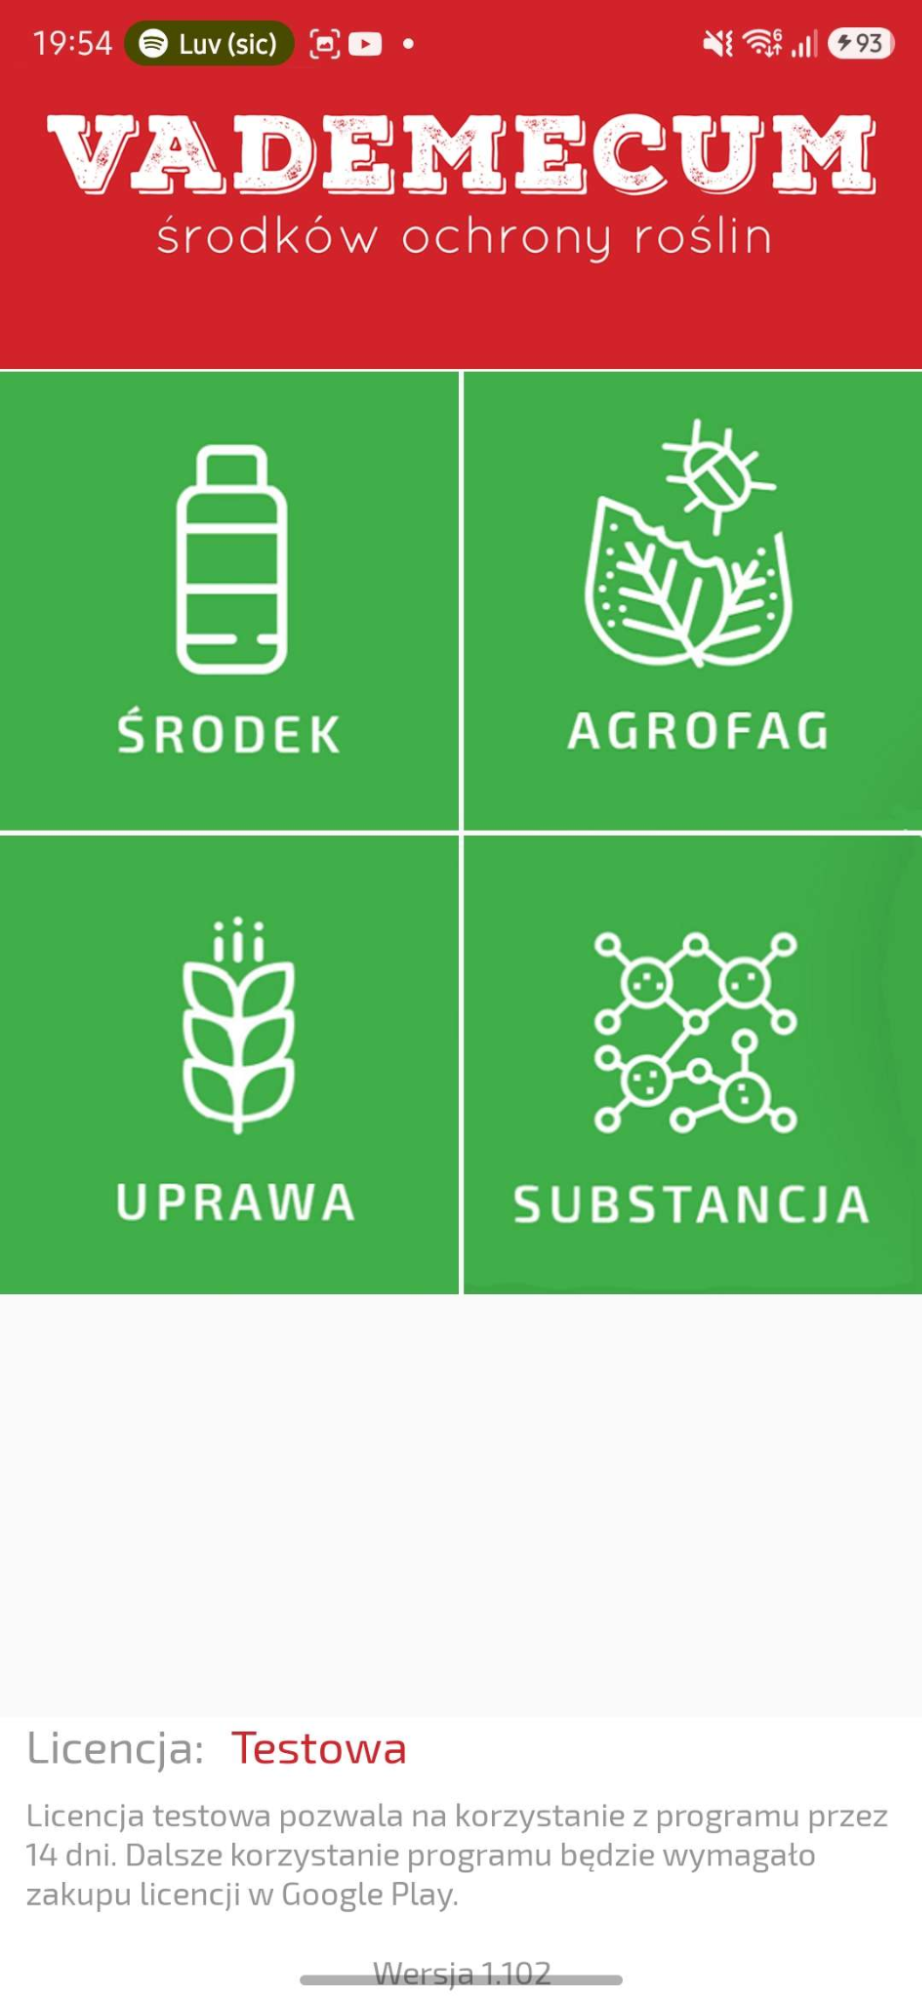
\includegraphics[width=0.3\linewidth]{vademecum1}
    \end{center}

    \item \textbf{Interfejs nieprzystosowany do obsługi w~terenie.}
    Problemy opisano na przykładzie wyszukiwania środka (zrzuty poniżej) --
    pozostałe wyszukiwarki korzystają z~tych samych komponentów.
    Baner reklamowy nachodzi na systemowy pasek stanu, zasłaniając m.in.
    aktualną godzinę. Przyciski powrotu znajdują się bardzo blisko dolnej
    krawędzi ekranu, więc zamiast cofnąć się do menu głównego użytkownik może
    przypadkowo wyjść z~aplikacji. Odstępy między polami wyszukiwania są
    bardzo małe, co zwiększa ryzyko wybrania niewłaściwego pola, a~same pola
    mają niespójny styl (zaokrąglenie tylko po lewej stronie). Przy obsłudze
    telefonu w~kabinie ciągnika takie elementy szczególnie sprzyjają
    pomyłkom.

    \begin{center}
        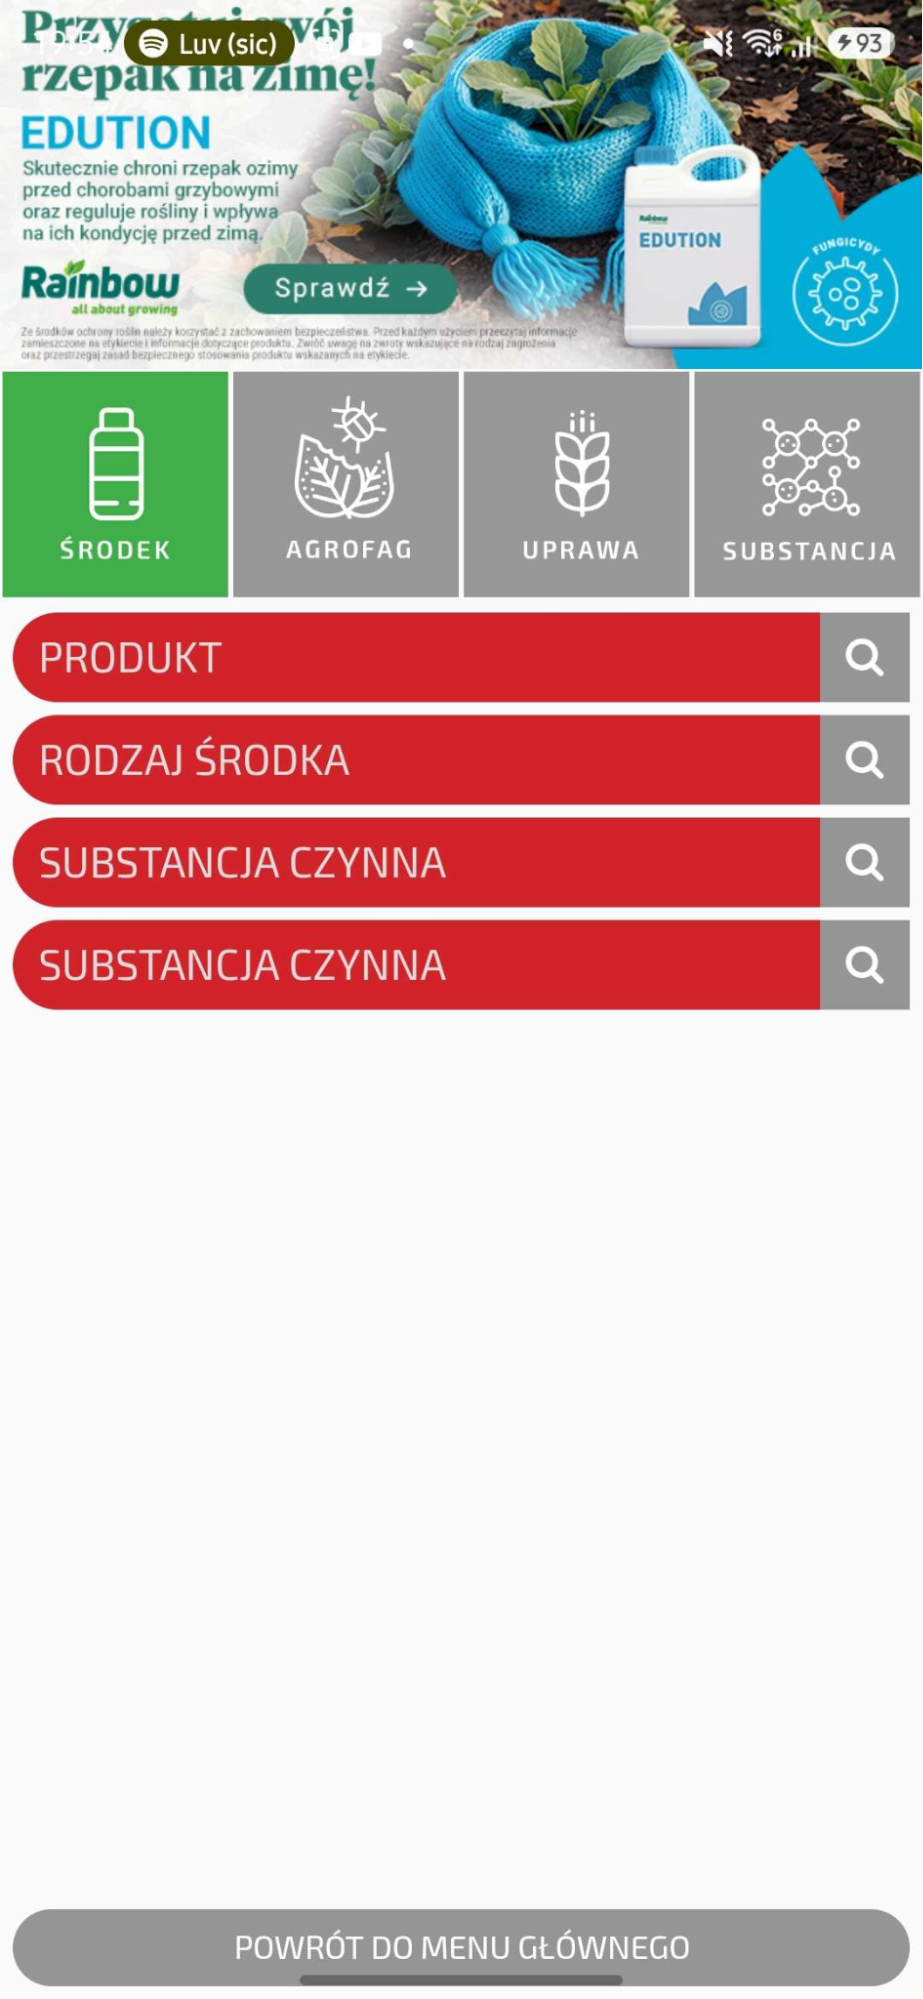
\includegraphics[width=0.3\linewidth]{vademecum2}\hfill
        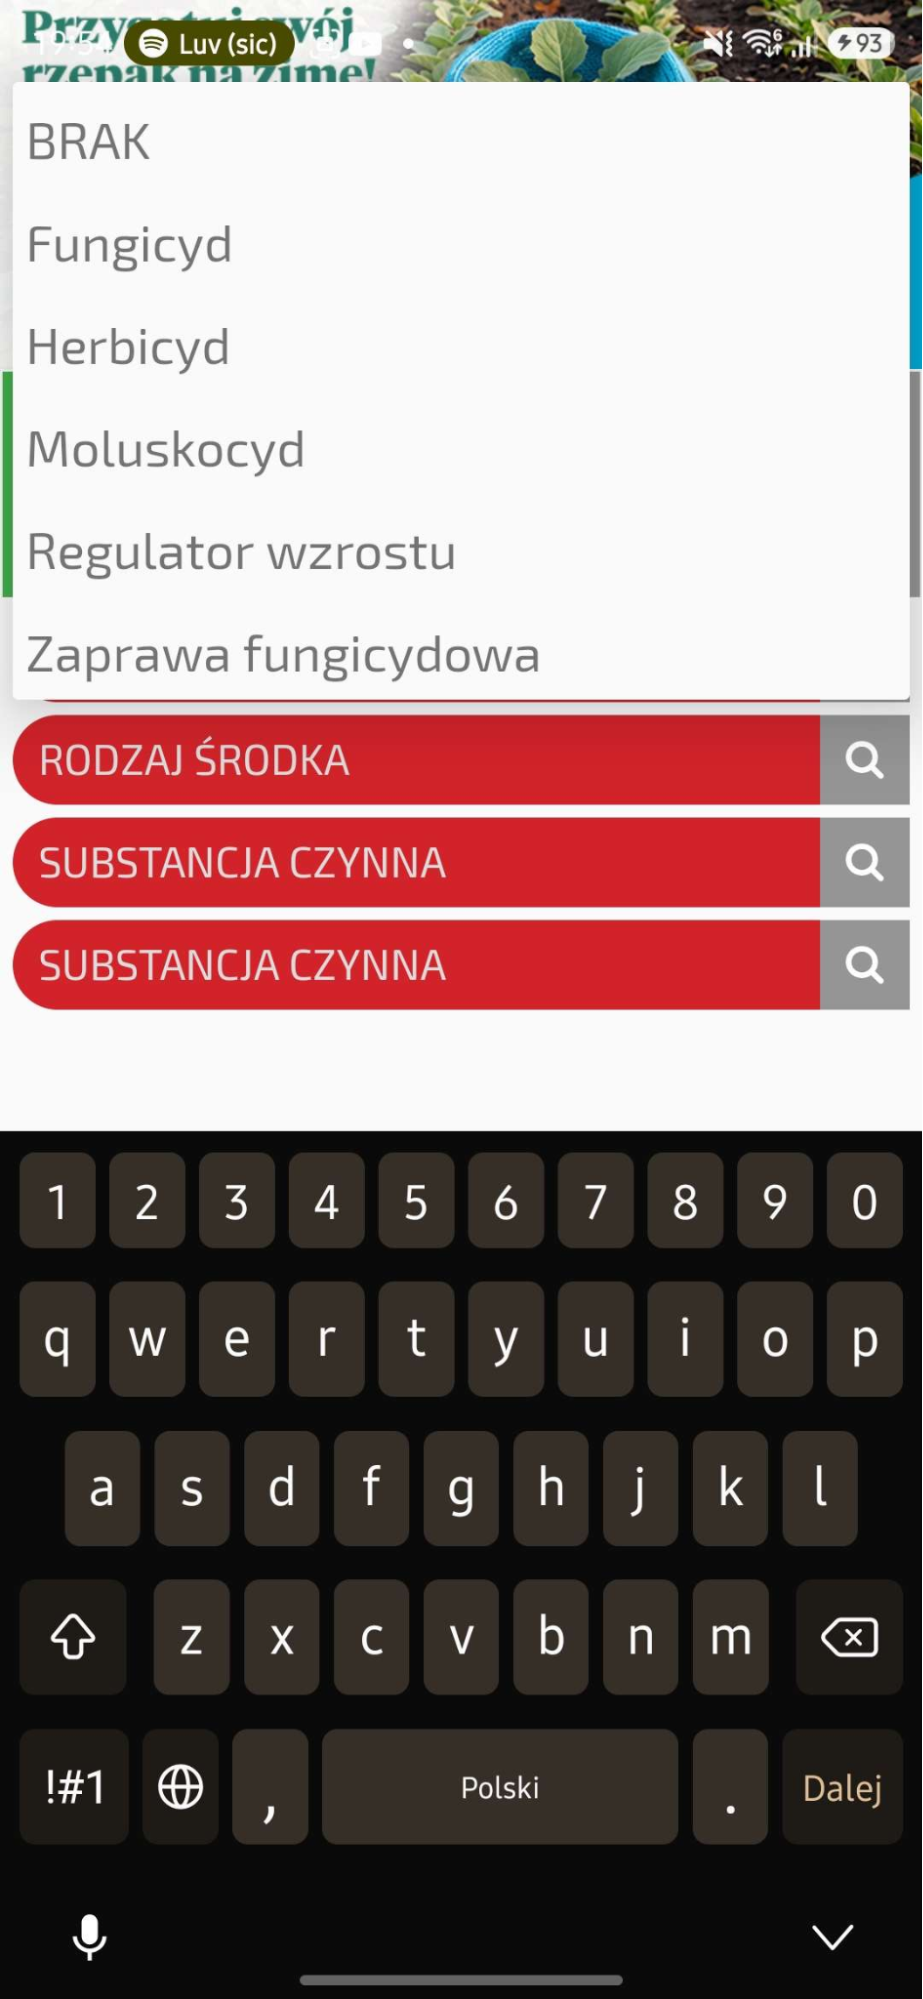
\includegraphics[width=0.3\linewidth]{vademecum3}\hfill
        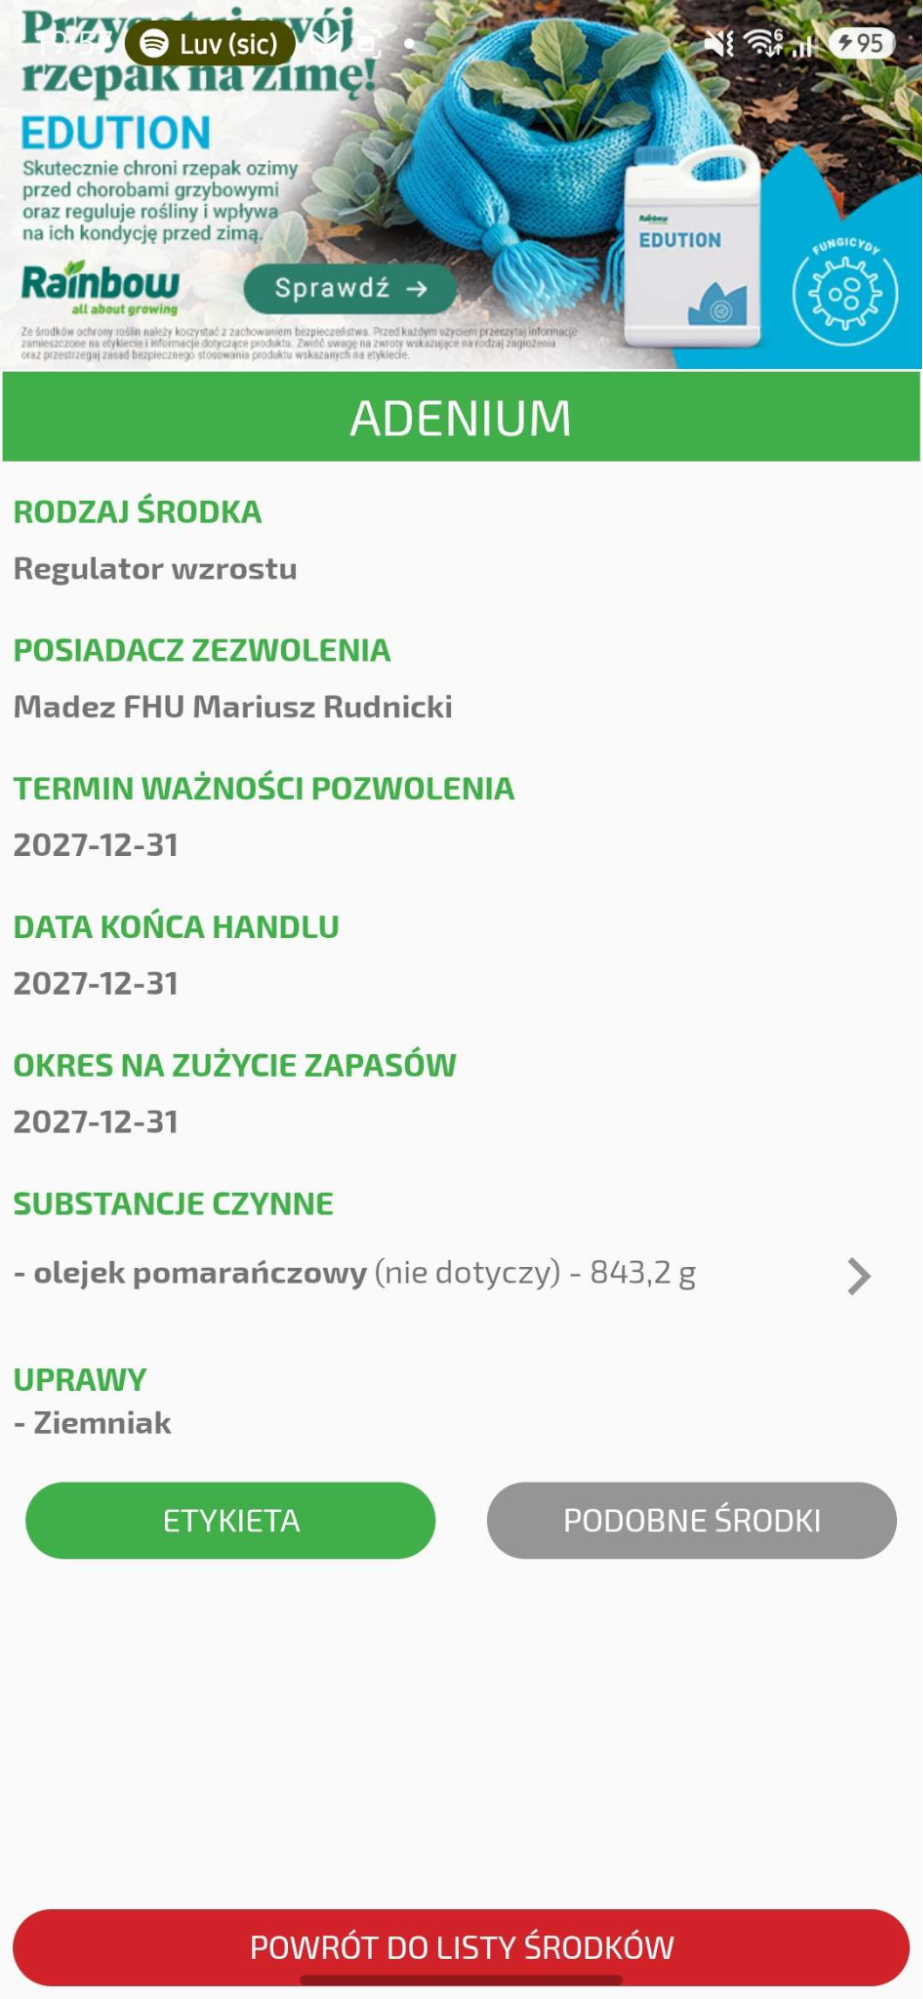
\includegraphics[width=0.3\linewidth]{vademecum4}
    \end{center}

    \item \textbf{Reklamy producentów środków.}
    Aplikacja wyświetla reklamy (w~sklepie Google Play ma oznaczenie
    ,,Zawiera reklamy'') -- na zrzutach widoczny jest baner reklamujący
    środek jednego z~producentów.

    \item \textbf{Etykieta pobierana bez podglądu.}
    Przycisk ,,Etykieta'' od razu pobiera plik na urządzenie, zamiast
    wyświetlić etykietę w~aplikacji z~osobną opcją pobrania. Użytkownik,
    który kilka razy sprawdza tę samą informację, nie wiedząc, że plik został
    już zapisany, może mieć w~telefonie np. cztery kopie tej samej etykiety.

    \item \textbf{Ograniczone możliwości wyszukiwania.}
    Wyszukiwarka nie toleruje literówek, nie pozwala łączyć filtrów (np.
    jednoczesnego wyboru uprawy i~agrofaga) ani ograniczyć wyników do
    środków dla użytkowników nieprofesjonalnych. Karta środka nie zawiera
    też okresu karencji.
\end{itemize}

\subsubsection{Wnioski dla projektu}

\begin{itemize}
    \item \textbf{Zachować:} cztery punkty wejścia do wyszukiwania oraz
    terminy prawne na karcie środka.
    \item \textbf{Nie powtarzać:} ograniczenia do jednej platformy, reklam,
    pobierania etykiety bez podglądu oraz elementów sterujących przy
    krawędziach ekranu.
    \item \textbf{Zrobić lepiej:} bezpłatny dostęp w~przeglądarce, podgląd
    etykiety w~aplikacji, okres karencji na karcie środka, duże elementy
    dotykowe z~odstępami oraz wyszukiwanie odporne na literówki z~możliwością
    łączenia filtrów.
\end{itemize}

\subsection{Wyszukiwarka środków ochrony roślin Ministerstwa Rolnictwa}

\subsubsection{Opis rozwiązania}

Ministerstwo Rolnictwa i~Rozwoju Wsi udostępnia na portalu gov.pl bezpłatną
wyszukiwarkę środków ochrony roślin. Według opisu ministerstwa pozwala ona
wyszukiwać środki ,,przede wszystkim po uprawach i~agrofagach'', a~także po
substancji czynnej, rodzaju środka oraz zastosowaniach
małoobszarowych.
Wyniki prezentowane są w~formie tabeli z~12 kolumnami, w~której każdy wiersz
opisuje jedno zastosowanie środka (środek, uprawa i~agrofag). Tabela zawiera
m.in. numer zezwolenia, rodzaj środka, substancję czynną z~zawartością, metodę
stosowania oraz rodzaj użytkownika (profesjonalny lub amatorski). Pozostałe
informacje -- terminy ważności zezwolenia i~dopuszczenia do sprzedaży
i~stosowania, dawka oraz termin stosowania -- są dostępne dopiero po wybraniu
opcji ,,zobacz szczegóły'' przy danym wierszu. Ministerstwo
udostępnia również plik źródłowy wyszukiwarki w~formacie XLSX, a~etykiety
środków -- na osobnej podstronie portalu. Formularz wyszukiwarki z~rozwiniętymi
filtrami przedstawiono poniżej.

\begin{center}
    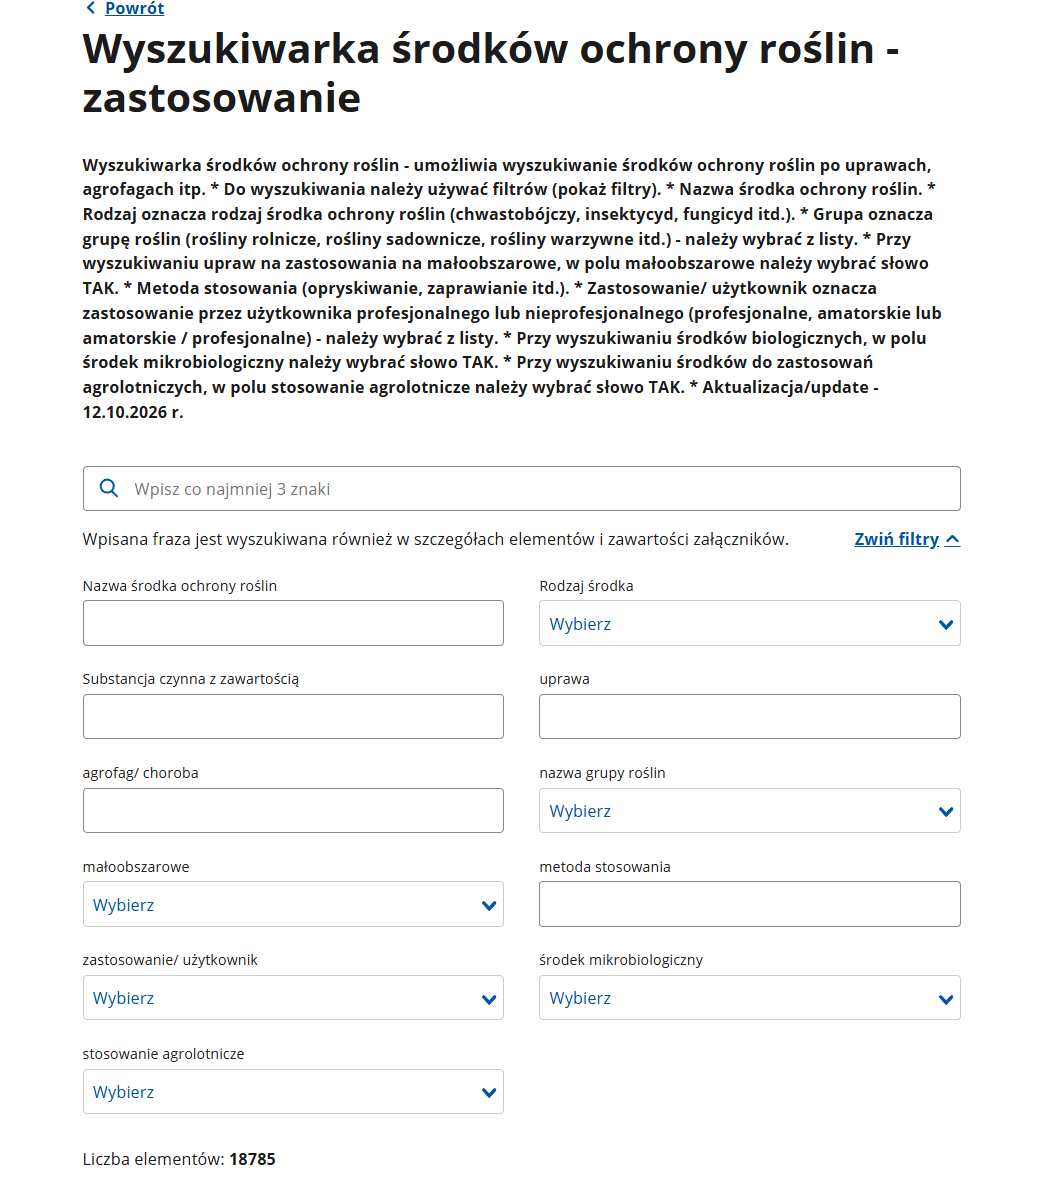
\includegraphics[width=0.72\textwidth]{GOV1}
\end{center}

\subsubsection{Mocne strony}

\begin{itemize}
    \item \textbf{Oficjalne i~bezpłatne źródło danych.}
    Dane pochodzą bezpośrednio od organu wydającego zezwolenia, a~korzystanie
    z~wyszukiwarki nie wymaga instalacji, logowania ani opłat.

    \item \textbf{Łączenie kryteriów wyszukiwania.}
    Większość kolumn ma własne pole filtra, dzięki czemu można jednocześnie
    zawęzić wyniki np. do konkretnej uprawy, agrofaga i~rodzaju środka.

    \item \textbf{Informacja o~rodzaju użytkownika.}
    Kolumna ,,zastosowanie/ użytkownik'' pozwala ograniczyć wyniki do
    zastosowań dopuszczonych dla użytkowników nieprofesjonalnych. W~danych
    pobranych 12~października 2026~r. na ok.~18,8~tys. zastosowań 346
    oznaczono jako wyłącznie amatorskie, a~ok.~1,5~tys. jako amatorskie
    i~profesjonalne.

    \item \textbf{Widoczna data aktualizacji.}
    W~opisie nad formularzem podana jest data ostatniej aktualizacji danych
    (12.10.2026~r.), dzięki czemu użytkownik wie, czy korzysta z~aktualnych
    informacji.
\end{itemize}

\subsubsection{Słabe strony}

\begin{itemize}
    \item \textbf{Pobieranie całej bazy przy każdym otwarciu.}
    Strona wyszukiwarki zawiera wszystkie zastosowania środków -- w~dniu
    analizy miała rozmiar ok.~10~MB. Przy słabym zasięgu w~polu wydłuża to
    wczytywanie strony i~zużywa pakiet danych użytkownika.

    \item \textbf{Zwielokrotnione wyniki.}
    Ministerstwo samo zaznacza, że ponieważ wyszukiwarka jest ,,zaprojektowana
    głównie pod uprawy'', w~wynikach ,,mogą pojawiać się zwielokrotnione nazwy
    środków ochrony roślin''. Użytkownik szukający informacji o~jednym środku
    musi przeglądać wiele wierszy zamiast jednej karty środka. Na zrzucie
    poniżej środek 3C-750 zajmuje sześć kolejnych wierszy -- po jednym dla
    każdej uprawy. Domyślnie wyświetlanych jest 10 wierszy na stronę, co przy
    18\,785 zastosowaniach daje 1879 stron wyników.

    \begin{center}
        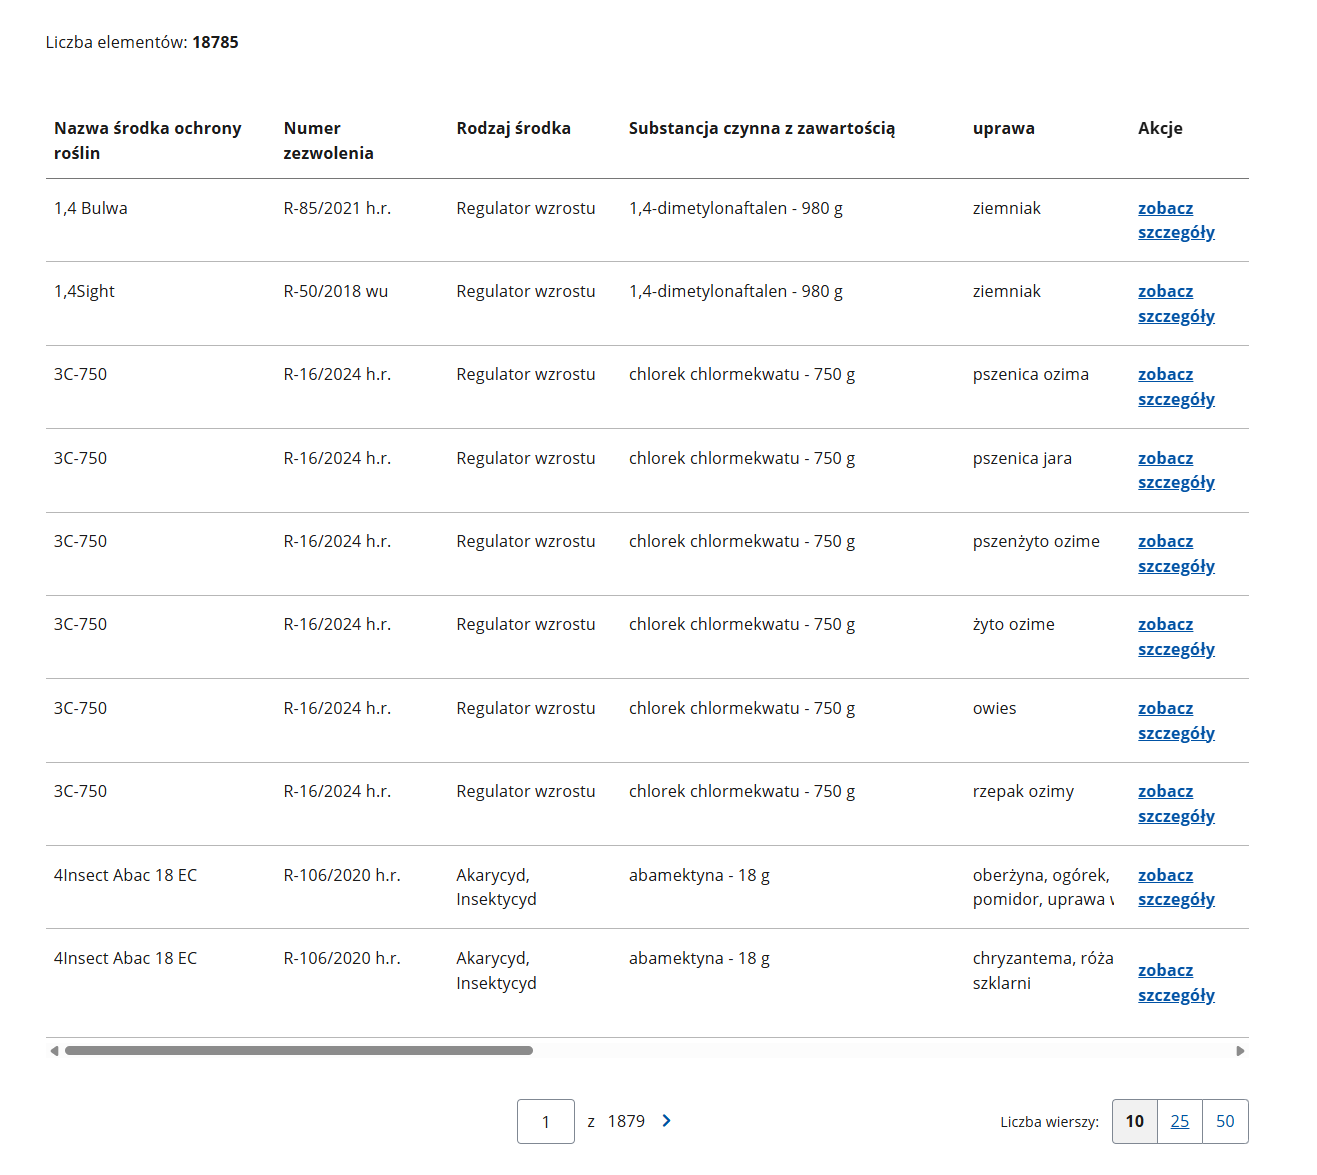
\includegraphics[width=0.85\textwidth]{GOV2}
    \end{center}

    \item \textbf{Etykieta poza wynikami.}
    Wyniki nie zawierają odnośników do etykiet -- aby zapoznać się z~etykietą,
    użytkownik musi przejść na osobną stronę z~etykietami i~odnaleźć tam
    właściwy dokument. Okres karencji jest podawany w~karcie produktu.
    Widok szczegółów pojedynczego zastosowania przedstawiono poniżej.

    \begin{center}
        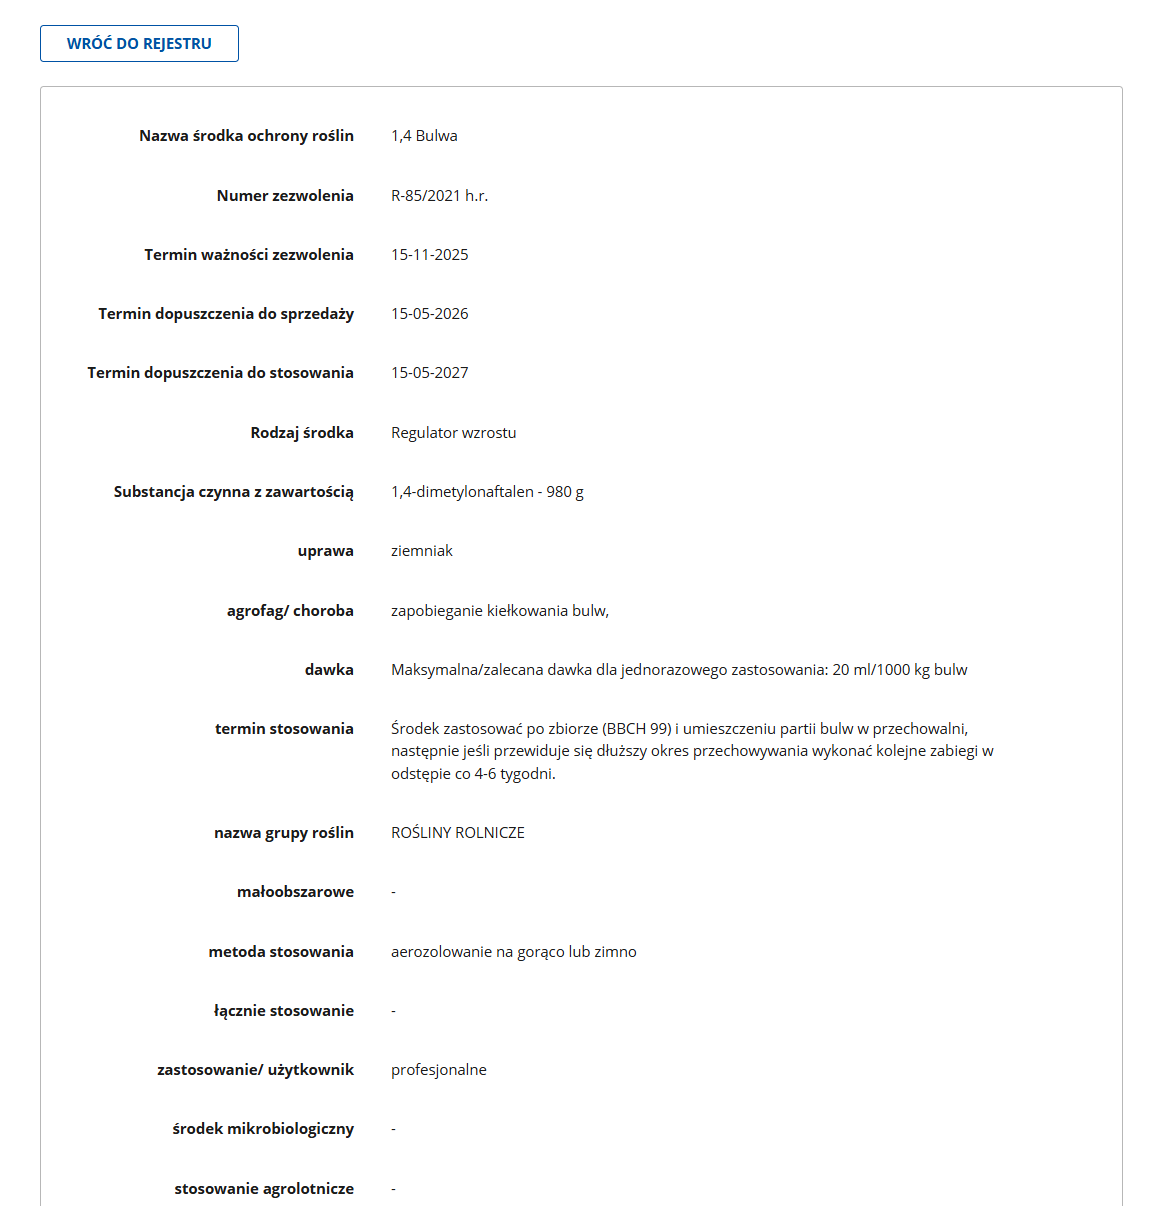
\includegraphics[width=0.85\linewidth]{GOV3}
    \end{center}

    \item \textbf{Tabela szersza niż ekran.}
    Tabela wyników nie mieści się w~całości nawet na monitorze komputera
    i~wymaga przewijania w~poziomie. Na zrzutach poniżej przedstawiono tę samą
    stronę wyników po przewinięciu tabeli do środka i~do prawej krawędzi.
    Kolumna ,,zastosowanie/ użytkownik'', kluczowa dla ogrodnika amatora,
    jest widoczna dopiero po przewinięciu tabeli do samego końca.

    \begin{center}
        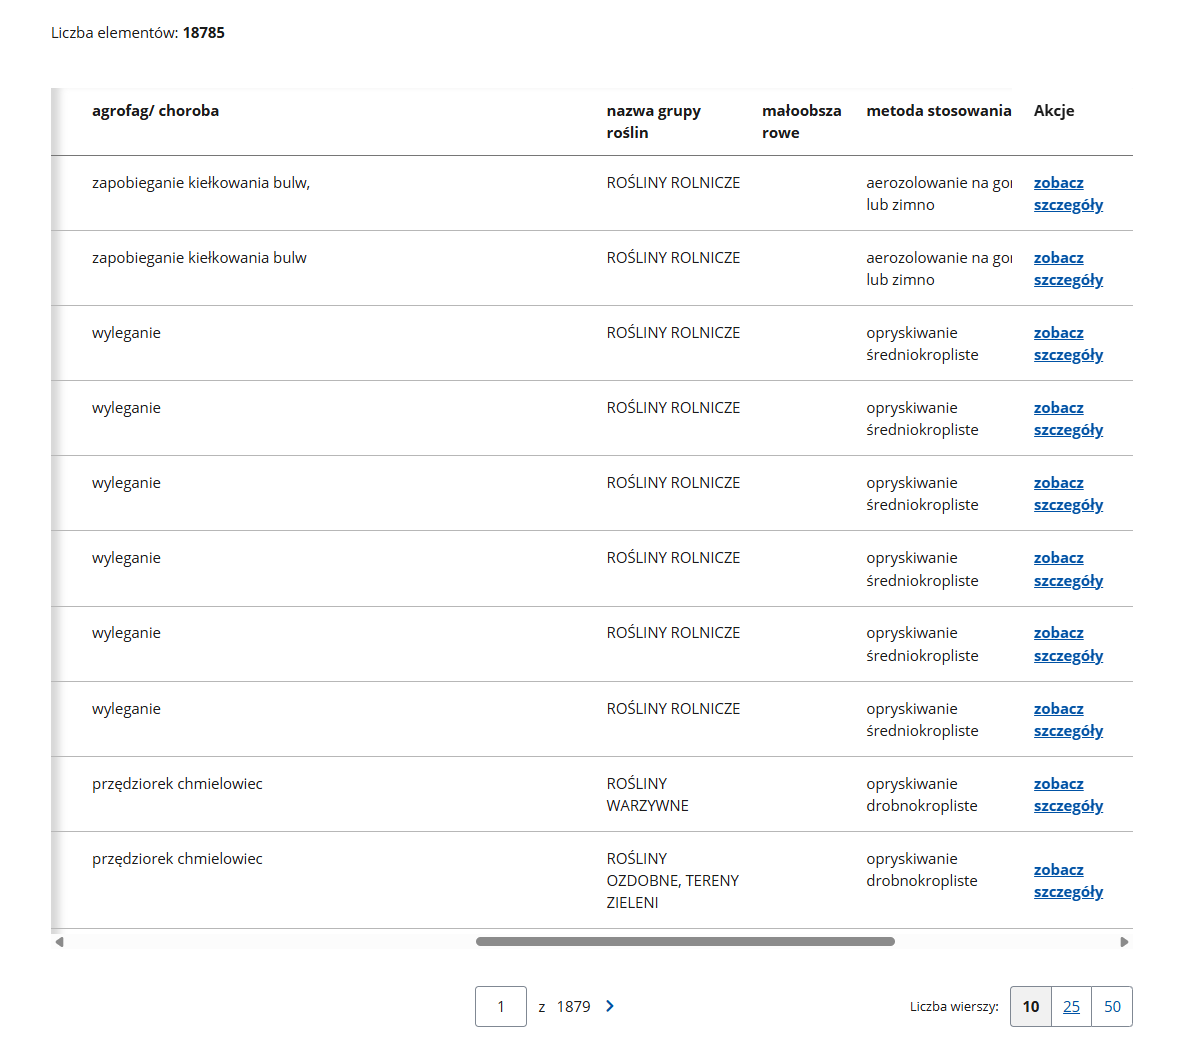
\includegraphics[width=0.9\linewidth]{GOV5}

        \vspace{0.5em}
        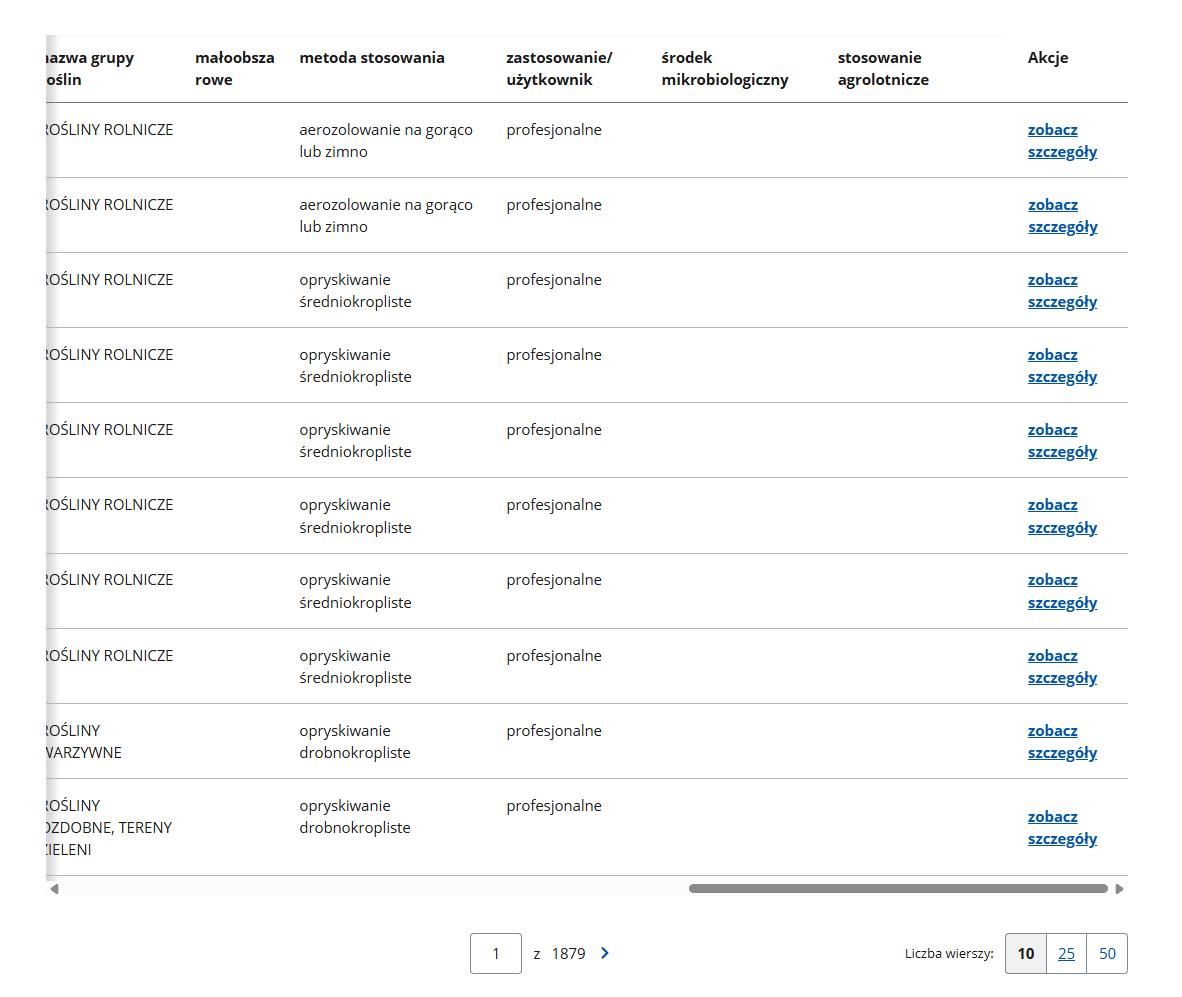
\includegraphics[width=0.9\linewidth]{GOV6}
    \end{center}

    \newpage
    Na ekranie telefonu problem jest jeszcze wyraźniejszy: widoczne są
    jedynie dwie pierwsze kolumny tabeli (nazwa środka i~numer zezwolenia),
    a~pozostałe, w~tym rodzaj środka i~uprawa, wymagają przewijania
    w~poziomie. Ponadto nad wynikami znajduje się formularz kilkunastu
    filtrów, który trzeba przewinąć, aby dotrzeć do tabeli.

    \begin{center}
        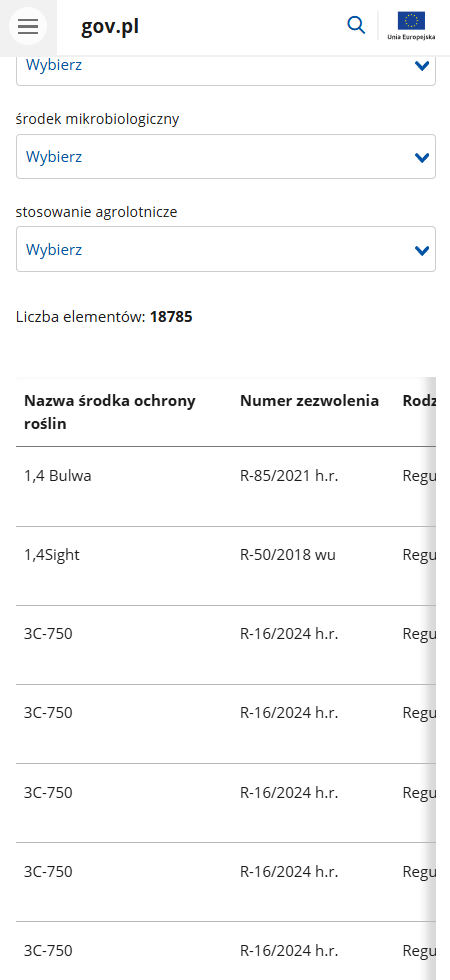
\includegraphics[height=12cm]{GOV4}
    \end{center}

    \item \textbf{Brak tolerancji literówek.}
    Wyszukiwarka dopasowuje wyłącznie dokładnie wpisany fragment tekstu.
    Podczas testów wpisanie nazwy środka z~literówką nie pozwoliło go
    odnaleźć. Jest to szczególnie uciążliwe przy nazwach handlowych, które
    często zawierają cyfry, skróty i~nietypową pisownię (np. ,,1,4Sight'',
    ,,3C-750'').
\end{itemize}

\subsubsection{Wnioski dla projektu}

\begin{itemize}
    \item \textbf{Zachować:} osobne filtry dla uprawy, agrofaga i~rodzaju
    środka oraz informację o~rodzaju użytkownika. Pliki CSV/XLSX publikowane
    przez ministerstwo na portalu dane.gov.pl mogą posłużyć jako źródło
    danych dla mechanizmu automatycznej aktualizacji.
    \item \textbf{Nie powtarzać:} przesyłania całej bazy do przeglądarki
    oraz wielokrotnego wyświetlania tego samego środka.
    \item \textbf{Zrobić lepiej:} wyniki pogrupowane według środka, karta
    środka z~odnośnikiem do etykiety i~wyróżnionym okresem karencji.
\end{itemize}

\newpage
\subsection{AgroBase}

\subsubsection{Opis rozwiązania}

AgroBase to międzynarodowa aplikacja litewskiej firmy Farmis, łącząca bazę
wiedzy o~agrofagach (chwastach, chorobach i~szkodnikach) z~bazą środków
ochrony roślin zarejestrowanych w~wybranym kraju. Jest dostępna na Androida
(ponad 500~tys. pobrań w~sklepie Google Play) i~iOS oraz w~wersji
przeglądarkowej z~osobną sekcją dla Polski. Interfejs obsługuje 45 języków,
w~tym polski. Wyszukiwarka w~podstawowej wersji jest bezpłatna i~zawiera
reklamy. Dodatkowe funkcje, takie jak lista ostatnio wybieranych środków,
wymagają subskrypcji w~cenie 16,99~zł miesięcznie lub 5,25~zł miesięcznie
przy płatności za rok z~góry. Jest to subskrypcja samej wyszukiwarki, a~nie
całego systemu AgroBase.

Użytkownik może wyszukać środek po nazwie, substancji czynnej, kategorii
lub uprawie albo zacząć od rozpoznania agrofaga na podstawie opisów
i~zdjęć, a~następnie przejść do środków, które go zwalczają. Karta środka
zawiera m.in. producenta, numer rejestracyjny, datę ważności rejestracji,
substancję czynną, odnośnik do etykiety oraz tabelę upraw z~dawką,
terminem stosowania (BBCH) i~okresem karencji. Dostępna jest także funkcja
porównania środków oraz zgłaszania błędów w~danych.

\subsubsection{Mocne strony}

\begin{itemize}
    \item \textbf{Wszystkie kluczowe informacje na jednej karcie.}
    Dawka, termin stosowania i~okres karencji są przedstawione w~jednej
    tabeli dla każdej uprawy, a~karta środka zawiera odnośnik do etykiety
    (choć nie zawsze działający -- zob. słabe strony). W~Vademecum etykietę
    trzeba pobrać jako plik, a~okresu karencji na karcie środka nie ma.
    W~wyszukiwarce ministerstwa okres karencji jest podawany w~karcie
    produktu, ale etykieta znajduje się na osobnej stronie.

    \item \textbf{Powiązanie agrofaga ze środkiem.}
    Rolnik, który nie zna nazwy szkodnika lub choroby, może najpierw
    rozpoznać go na podstawie zdjęć i~opisu, a~dopiero potem wyszukać
    środki, które go zwalczają.

    \item \textbf{Trzy platformy.}
    Aplikacja działa na Androidzie, iOS oraz w~przeglądarce.
\end{itemize}

\subsubsection{Słabe strony}

\begin{itemize}
    \item \textbf{Tłumaczenie maszynowe.}
    Polskie teksty zawierają błędy wskazujące na automatyczne tłumaczenie,
    np. na karcie środka ,,Aktywne materiały'' zamiast ,,substancje
    czynne'', ,,Stawka'' zamiast ,,dawka'' czy ,,Karencji interwał'',
    a~w~opisie aplikacji w~sklepie Google Play ,,Dokonywanie harcerstwa
    w~terenie'' (z~ang. \emph{scouting} -- lustracja pól). Terminologia
    niezgodna z~etykietami utrudnia zrozumienie danych i~obniża zaufanie
    do nich.

    \item \textbf{Wątpliwa jakość części danych.}
    Na karcie środka Amistar 250 SC dla słodkiej papryki podano dawkę
    ,,0~l'', co wskazuje na błąd w~danych. Aplikacja nie jest oficjalnym
    źródłem, a~producent sam prosi użytkowników o~zgłaszanie błędnych
    informacji.

    \item \textbf{Nieaktualna baza środków.}
    Polska sekcja wersji przeglądarkowej zawiera 1797 środków. Porównanie
    ich nazw z~danymi wyszukiwarki ministerstwa, przeprowadzone
    13~października 2026~r., wykazało, że w~aktualnym rejestrze występuje jedynie od 935 do ok.~1130
    z~nich (52--63\,\%, zależnie od sposobu dopasowania nazw). Pozostałych
    środków nie ma w~aktualnym rejestrze -- na stronie głównej listy
    wyświetlane są np. Arcade 880 EC, którego rejestracja według samej
    aplikacji wygasła 4~marca 2026~r., oraz Maxim Star 025 FS, również
    z~wygasłą rejestracją. Aplikacja nie pozwala odfiltrować takich środków.
    Jednocześnie aktywne środki w~AgroBase to zaledwie ok.~jedna trzecia
    z~ok.~3~tys. środków występujących w~danych ministerstwa, więc
    użytkownik może nie znaleźć w~aplikacji środka, który jest dopuszczony
    do stosowania.

    \item \textbf{Nieneutralna kolejność środków.}
    Lista środków nie jest uporządkowana alfabetycznie -- na jej początku
    wyświetlane są produkty firm Bayer i~Syngenta. Na zrzucie poniżej
    widać początek listy: pierwszym środkiem jest Arcade 880 EC z~wygasłą
    rejestracją, a~kolejne pozycje to wyłącznie produkty tych dwóch firm.

    \begin{center}
        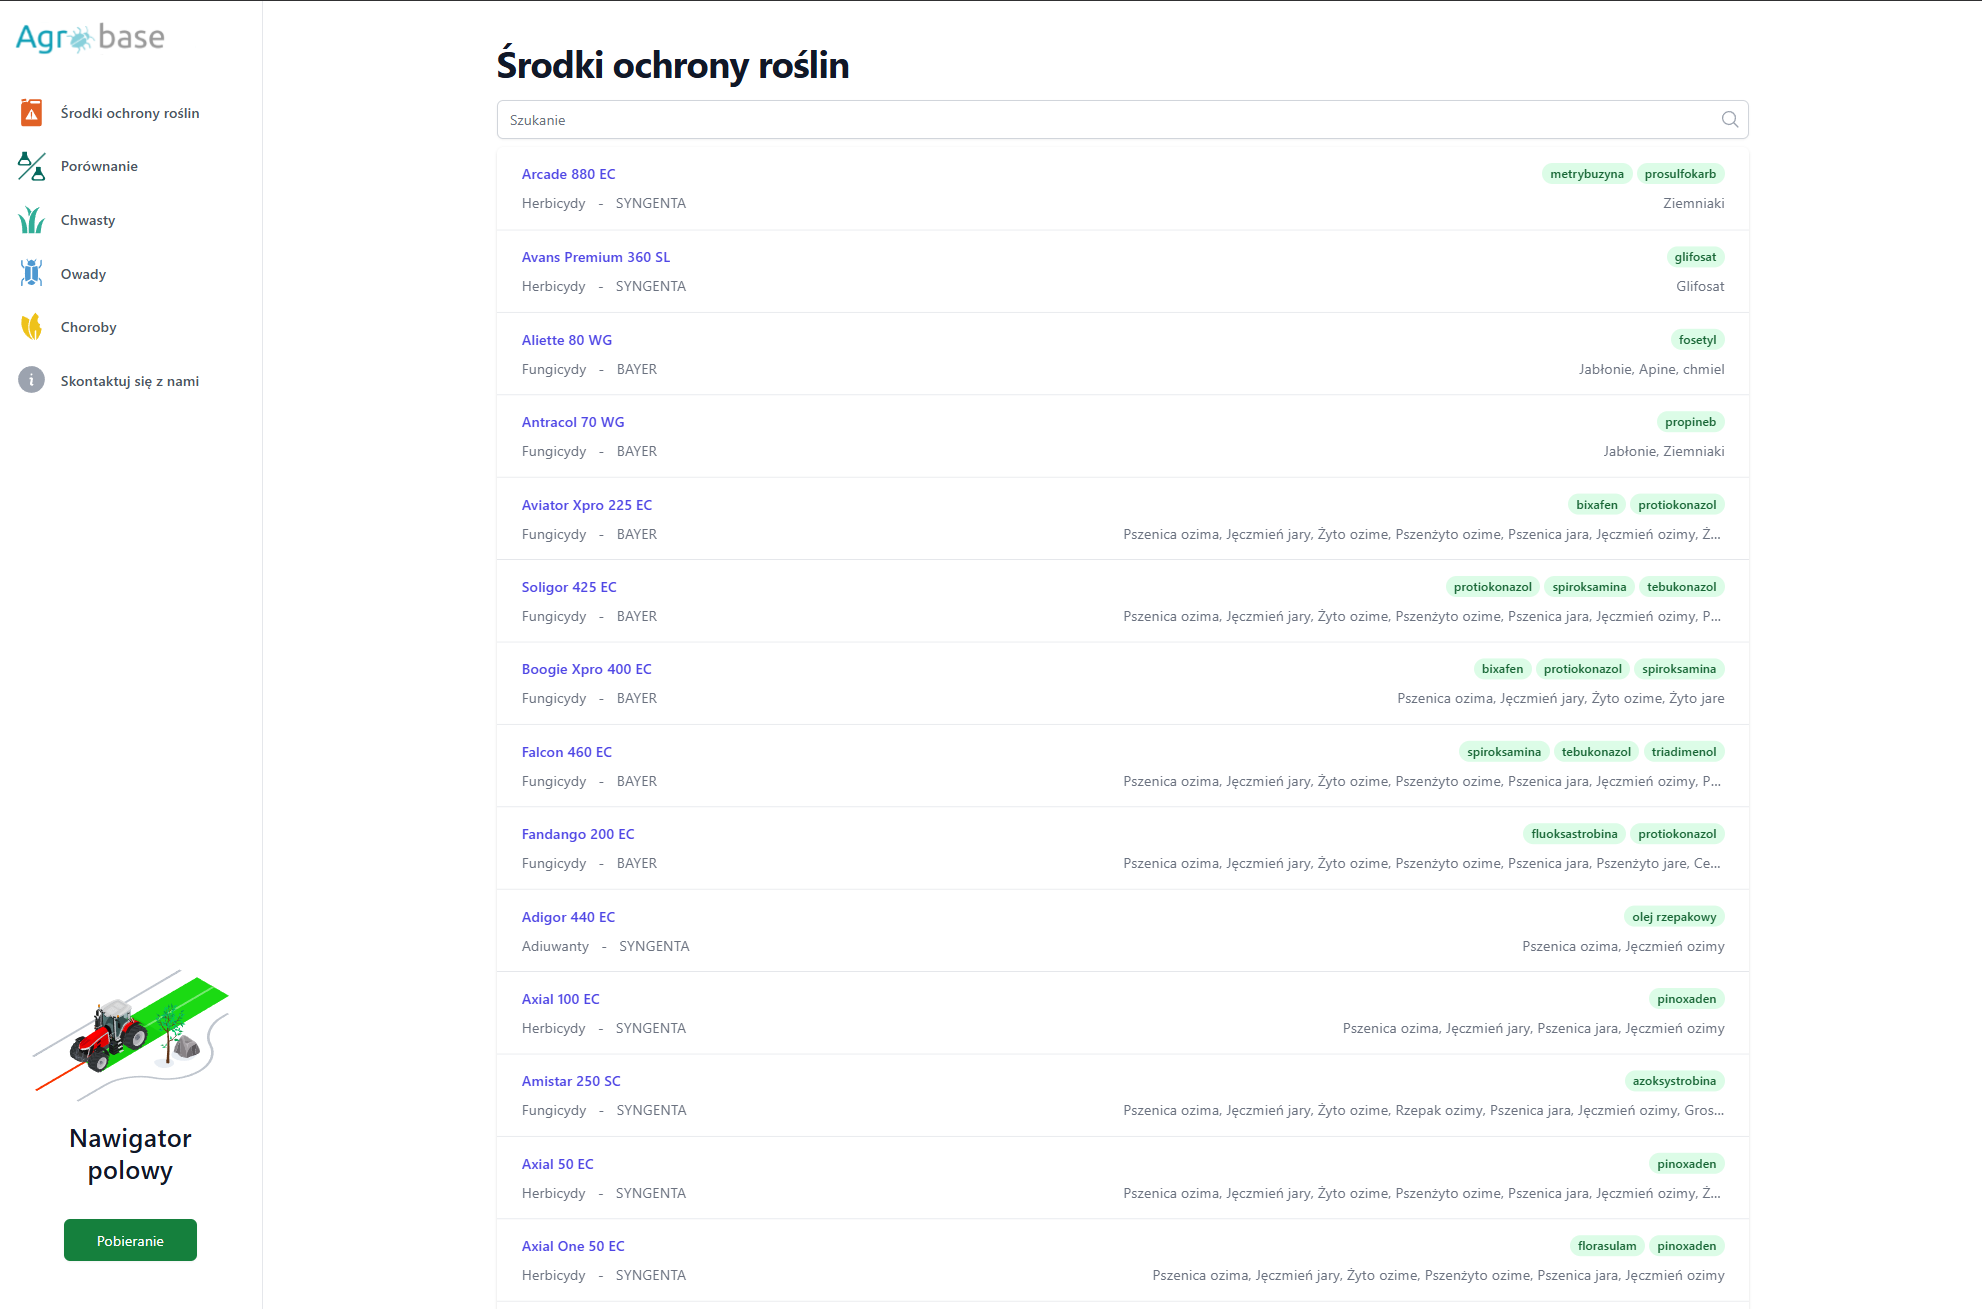
\includegraphics[width=\linewidth]{AgroBase1}
    \end{center}

    \item \textbf{Niedziałające odnośniki do etykiet.}
    Odnośniki do etykiet i~kart charakterystyki prowadzą do różnych
    serwisów -- części do portalu gov.pl, części do stron producentów.
    Odnośniki do strony firmy Bayer zwracają błąd 404 (strona nie
    istnieje), np. etykieta środka Antracol 70 WG oraz karta
    charakterystyki środka Aliette 80 WG. Karta tego ostatniego środka
    (poniżej) pokazuje jednocześnie inne opisane problemy: datę wygaśnięcia
    rejestracji (14~marca 2026~r.) aplikacja wyróżnia kolorem czerwonym,
    ale nadal prezentuje środek, a~substancja czynna opisana jest jako
    ,,Aktywne materiały''.

    \begin{center}
        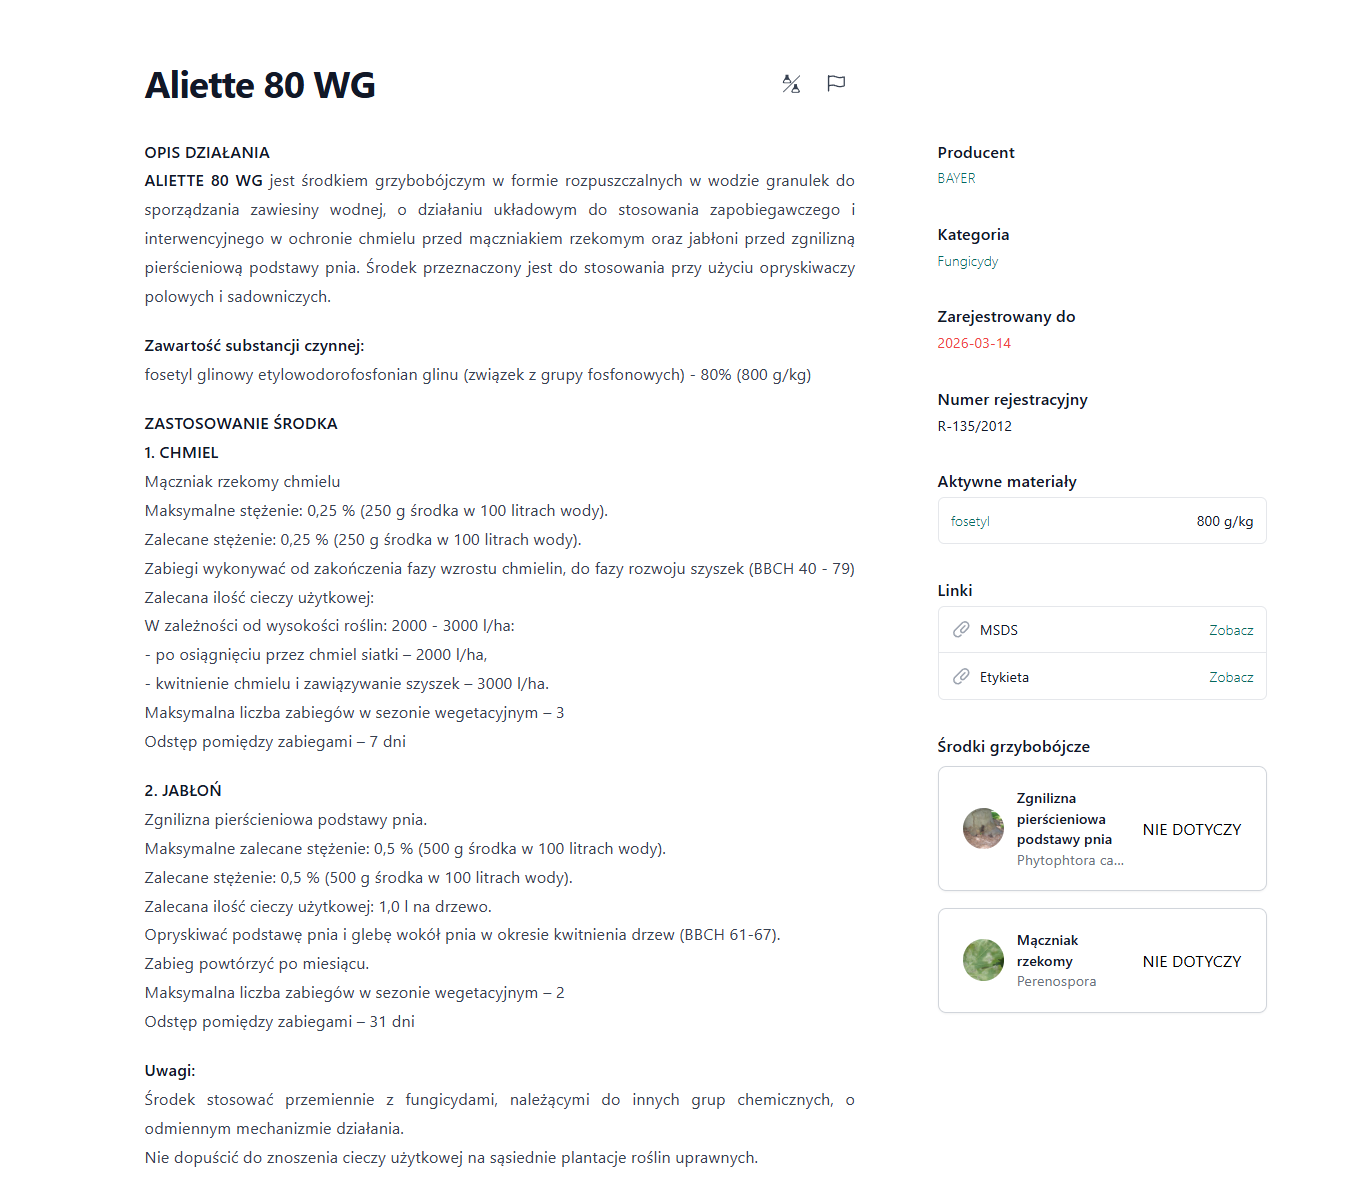
\includegraphics[width=\linewidth]{AgroBase2}
    \end{center}

    \item \textbf{Niepełne informacje prawne.}
    Karta środka podaje jedynie datę ważności rejestracji -- brakuje
    terminów dopuszczenia do sprzedaży i~stosowania, które są dostępne
    w~Vademecum i~w~wyszukiwarce ministerstwa.

    \item \textbf{Ograniczone możliwości wyszukiwania.}
    Wyszukiwarka nie toleruje literówek, nie pozwala łączyć filtrów
    (np. jednoczesnego wyboru uprawy i~agrofaga) ani ograniczyć wyników do
    środków dopuszczonych dla użytkowników nieprofesjonalnych.

    \item \textbf{Reklamy i~płatne subskrypcje.}
    Bezpłatna wersja wyświetla reklamy, a~nawet tak podstawowe udogodnienia
    jak lista ostatnio wybieranych środków wymagają subskrypcji (16,99~zł
    miesięcznie lub 5,25~zł miesięcznie przy płatności rocznej).
\end{itemize}

\subsubsection{Wnioski dla projektu}

\begin{itemize}
    \item \textbf{Zachować:} kartę środka z~tabelą upraw zawierającą dawkę
    i~okres karencji oraz możliwość zgłoszenia błędu w~danych.
    \item \textbf{Nie powtarzać:} tłumaczenia maszynowego -- interfejs
    powinien używać terminologii zgodnej z~etykietami (substancja czynna,
    dawka, okres karencji).
    \item \textbf{Zrobić lepiej:} dane pobierane bezpośrednio z~oficjalnego
    źródła (ministerstwa) i~regularnie aktualizowane, tak aby nie
    wyświetlać środków z~wygasłą rejestracją; pełne terminy prawne, data
    aktualizacji oraz etykiety pochodzące z~portalu gov.pl zamiast
    z~zewnętrznych serwisów producentów.
\end{itemize}

\subsection{Porównanie funkcji}

\begin{center}
\footnotesize
\begin{tabular}{|p{3.5cm}|p{2.8cm}|p{2.8cm}|p{2.5cm}|p{1.9cm}|}
\hline
\textbf{Funkcja} & \textbf{Vademecum} & \textbf{MRiRW} & \textbf{AgroBase} & \textbf{Projekt} \\
\hline
Platformy & Android & przeglądarka & Android, iOS, przeglądarka & przeglądarka \\
\hline
Koszt & 119 zł/rok (odnowienie 139 zł) lub 829 zł & bezpłatne & bezpłatne z~reklamami; subskrypcja 16,99~zł/mies. lub 5,25~zł/mies. rocznie & bezpłatne \\
\hline
Wyszukiwanie po nazwie, uprawie, agrofagu, substancji & tak & tak & tak & tak \\
\hline
Łączenie filtrów (uprawa + agrofag) & nie & tak & nie & tak \\
\hline
Tolerancja literówek & nie & nie & nie & tak \\
\hline
Filtr środków dla amatorów & nie & tak & nie & tak \\
\hline
Podgląd etykiety w~aplikacji & nie (pobranie pliku) & nie (osobna strona) & nie (odnośnik zewnętrzny, część nie działa) & tak \\
\hline
Okres karencji na karcie środka & nie & tak & tak & tak \\
\hline
Terminy prawne & tak & tak & tylko ważność rejestracji & tak \\
\hline
Reklamy & tak & nie & tak & nie \\
\hline
\end{tabular}
\end{center}

Różnice w~funkcjach wynikają przede wszystkim z~celu, w~jakim powstało każde
z~rozwiązań. Wyszukiwarka ministerstwa jest narzędziem urzędowym -- udostępnia
pełne dane z~rejestru, łącznie z~rzadko potrzebnymi informacjami (np.
stosowanie agrolotnicze), ale nie jest projektowana z~myślą o~telefonie ani
o~wygodzie przeglądania. Vademecum jest produktem komercyjnym, który sprzedaje
wygodny dostęp do tych samych danych -- stąd licencja, a~według karty
w~sklepie Google Play także reklamy. AgroBase jest produktem
międzynarodowym, obsługującym wiele krajów i~języków -- stąd szeroki zakres
(rozpoznawanie chwastów, chorób i~szkodników), ale też tłumaczenie maszynowe
i~brak części informacji specyficznych dla polskiego rejestru, takich jak
termin dopuszczenia do sprzedaży.

\subsection{Zidentyfikowane problemy użytkowników}

\begin{enumerate}
    \item \textbf{Dostęp do danych wymaga licencji lub pobrania całej bazy.}
    Vademecum działa wyłącznie na Androidzie i~po 14 dniach wymaga licencji,
    a~wyszukiwarka ministerstwa przy każdym otwarciu pobiera ok.~10~MB danych.

    \item \textbf{Interfejs utrudnia obsługę w~warunkach polowych.}
    Małe odstępy między polami i~przyciski przy krawędzi ekranu sprzyjają
    pomyłkom podczas obsługi telefonu w~kabinie ciągnika (Vademecum).

    \item \textbf{Etykieta jest poza wynikami wyszukiwania.}
    W~Vademecum etykieta jest pobierana jako plik i~otwierana w~innym
    programie, a~w~wyszukiwarce ministerstwa znajduje się na osobnej
    podstronie, bez odnośnika z~wyników. Vademecum nie pokazuje też okresu
    karencji -- aby go sprawdzić, trzeba odszukać go w~treści etykiety.
    W~AgroBase etykiety są dostępne przez odnośniki do zewnętrznych
    serwisów, z~których część nie działa.

    \item \textbf{Ten sam środek pojawia się w~wynikach wielokrotnie.}
    W~wyszukiwarce ministerstwa każdy wiersz to jedno zastosowanie, więc
    informacje o~jednym środku są rozproszone po wielu wierszach.

    \item \textbf{Literówka w~nazwie środka uniemożliwia jego znalezienie.}
    Żadne z~analizowanych rozwiązań nie odnajduje środka, jeśli jego nazwa
    zostanie wpisana z~błędem. Użytkownik musi znać dokładną pisownię nazwy
    handlowej, co w~terenie -- przy pisaniu na telefonie -- jest
    utrudnieniem.
\end{enumerate}

\subsection{Funkcje projektowanego systemu}

\begin{enumerate}
    \item \textbf{Wyszukiwanie odporne na literówki} po nazwie handlowej
    i~substancji czynnej.

    \item \textbf{Filtrowanie krzyżowe} -- jednoczesny wybór uprawy,
    agrofaga i~rodzaju środka, z~możliwością ograniczenia wyników do środków
    dla użytkowników nieprofesjonalnych.

    \item \textbf{Karta środka} grupująca wszystkie jego zastosowania,
    z~dawkowaniem, okresem karencji, terminami prawnymi oraz podglądem
    etykiety bezpośrednio w~aplikacji.

    \item \textbf{Wyszukiwanie zamienników} o~tej samej substancji czynnej
    i~stężeniu, z~uwzględnieniem zakresu stosowania (uprawa, agrofag) oraz
    tego, czy środek jest dopuszczony dla użytkowników nieprofesjonalnych.

    \item \textbf{Automatyczna aktualizacja danych} z~kwartalnie
    aktualizowanych plików CSV/XLSX publikowanych przez Ministerstwo
    Rolnictwa na portalu dane.gov.pl, z~widoczną dla użytkownika datą
    ostatniej aktualizacji.
\end{enumerate}

\subsection{Co projektowany system powinien robić lepiej}

\begin{enumerate}
    \item \textbf{Dostęp bez instalacji i~bez obciążania łącza.}
    Aplikacja webowa działa w~przeglądarce, więc -- w~przeciwieństwie do
    Vademecum -- nie wymaga instalacji. W~przeciwieństwie do
    wyszukiwarki ministerstwa przesyła do telefonu tylko wyniki zapytania,
    a~nie całą bazę danych.

    \item \textbf{Obsługa w~terenie.} Duże elementy dotykowe z~odstępami,
    nawigacja oddalona od krawędzi ekranu i~wysoki kontrast czytelny
    w~pełnym słońcu.

    \item \textbf{Zamienniki z~uwzględnieniem uprawnień.} Wyszukiwarka
    ministerstwa zawiera informację o~rodzaju użytkownika, ale nie wskazuje
    zamienników. Projektowany system łączy oba elementy: wskazuje środki
    o~tym samym składzie, które są zarejestrowane dla tej samej uprawy
    i~dopuszczone dla użytkownika nieprofesjonalnego.

    \item \textbf{Aktualność danych.} System będzie automatycznie
    aktualizował swoją bazę na podstawie kwartalnie aktualizowanych danych
    rządowych. Środki, których nie ma już w~rejestrze ministerstwa, nie
    będą prezentowane jako dostępne -- w~przeciwieństwie do AgroBase, gdzie
    na początku listy wyświetlane są środki z~wygasłą rejestracją, a~ok.
    37--48\,\% bazy stanowią środki nieobecne w~aktualnym rejestrze.
\end{enumerate}


\section{Cel projektu}

Celem projektu jest opracowanie i implementacja responsywnej
aplikacji internetowej pełniącej rolę inteligentnej wyszukiwarki
środków ochrony roślin. System ma umożliwić łatwy, darmowy,
niezależny i szybki dostęp do ujednoliconych danych o preparatach
rolniczych z poziomu urządzeń mobilnych.

\section{Proponowane rozwiązanie}

Planowane jest stworzenie systemu w formie aplikacji webowej z interfejsem dostosowanym do urządzeń
mobilnych zgodnie z podejściem \emph{Mobile First}.

System będzie automatycznie pobierał i aktualizował dane z rządowego
portalu otwartych danych dane.gov.pl, na którym Ministerstwo Rolnictwa
i~Rozwoju Wsi kwartalnie publikuje rejestr środków ochrony roślin oraz dane
wyszukiwarki środków ochrony roślin w~formatach CSV i~XLSX. Pliki będą
pobierane za pośrednictwem API portalu (api.dane.gov.pl).

Aplikacja udostępni wyszukiwarkę wykorzystującą mechanizm
wyszukiwania rozmytego (\emph{fuzzy search}), umożliwiający
uwzględnianie literówek oraz różnych wariantów nazw.

Użytkownik będzie mógł korzystać z krzyżowego filtrowania, np.
poprzez jednoczesny wybór uprawy i szkodnika, a także przeglądać
szczegółowe karty produktów zawierające informacje dotyczące
dawkowania oraz terminów stosowania.

\newpage
\section{Specyfikacja wymagań}
\label{sec:specyfikacja}

Specyfikacja opisuje, czego oczekujemy od systemu, bez przesądzania o~sposobie
jego realizacji. Wymagania funkcjonalne oznaczono identyfikatorami WF-xx,
a~niefunkcjonalne -- WNF-xx. Każde wymaganie ma przypisany priorytet:

\begin{itemize}
    \item \textbf{MUST} -- wymaganie konieczne; bez niego system nie realizuje
    swojego podstawowego celu,
    \item \textbf{SHOULD} -- wymaganie ważne, które powinno zostać zrealizowane,
    ale system może bez niego funkcjonować,
    \item \textbf{COULD} -- wymaganie dodatkowe, realizowane w~miarę dostępnego
    czasu.
\end{itemize}

\subsection{Zakres systemu}

System obejmuje:

\begin{itemize}
    \item wyszukiwanie środków ochrony roślin po nazwie handlowej, substancji
    czynnej, uprawie i~agrofagu, wraz z~filtrowaniem krzyżowym,
    \item kartę środka z~informacjami o~zastosowaniach, dawkach, terminach
    prawnych i~etykiecie,
    \item wyszukiwanie środków o~tych samych substancjach czynnych
    (zamienników),
    \item automatyczną aktualizację danych na podstawie publicznych danych
    Ministerstwa Rolnictwa i~Rozwoju Wsi.
\end{itemize}

Poza zakresem systemu są: ceny i~sprzedaż środków, konta użytkowników i~panel
administracyjny, ewidencja wykonanych zabiegów, rozpoznawanie agrofagów na
podstawie zdjęć, aplikacja instalowana na urządzeniu oraz praca bez dostępu do
internetu.

\subsection{Interesariusze}

\begingroup
\small
\begin{longtable}{|>{\raggedright\arraybackslash}p{3.2cm}|p{8.8cm}|>{\raggedright\arraybackslash}p{2.4cm}|}
\hline
\textbf{Interesariusz} & \textbf{Opis i~potrzeba} & \textbf{Wymagania} \\
\hline
\endfirsthead
\hline
\textbf{Interesariusz} & \textbf{Opis i~potrzeba} & \textbf{Wymagania} \\
\hline
\endhead
Doradca agronomiczny / rolnik profesjonalny &
Analizuje składy chemiczne środków, planuje rotację preparatów i~weryfikuje
ich zgodność z~aktualnym prawem oraz zasadami integrowanej ochrony roślin.
,,Chcę wiedzieć, czym mogę zastąpić środek i~czy jest on dopuszczony na moją
uprawę.'' &
WF-03, WF-04, WF-10, WF-16 \\
\hline
Rolnik indywidualny / operator maszyn &
Wykonuje zabiegi w~terenie i~sprawdza na smartfonie dawkowanie, warunki
stosowania oraz okresy karencji i~prewencji bezpośrednio z~kabiny ciągnika.
,,Chcę w~kabinie ciągnika sprawdzić dawkę i~karencję, nawet przy słabym
zasięgu.'' &
WF-06, WF-07, WNF-01 do WNF-05 \\
\hline
Ogrodnik amator / działkowiec &
Szuka bezpiecznych środków do upraw przydomowych, dostępnych bez uprawnień
profesjonalnych. ,,Chcę wiedzieć, których środków mogę legalnie używać
i~czy istnieją tańsze odpowiedniki drogiej, małej butelki ze sklepu
ogrodniczego.'' &
WF-05, WF-10 \\
\hline
Ministerstwo Rolnictwa i~Rozwoju Wsi &
Dostawca danych -- publikuje rejestr środków ochrony roślin na portalu
dane.gov.pl. Jego dane muszą być prezentowane bez zniekształceń, a~rytm ich
publikacji wyznacza rytm aktualizacji systemu. &
WF-13, WNF-07, O-01 \\
\hline
Zespół projektowy &
Twórcy i~opiekunowie systemu. ,,Chcemy, żeby dane aktualizowały się bez
naszej ręcznej pracy.'' &
WF-13, WNF-08, O-04 \\
\hline
Producenci i~dystrybutorzy środków (interesariusz pośredni) &
Ich produkty są prezentowane w~systemie, dlatego oczekują rzetelnej
i~neutralnej prezentacji. &
WNF-09 \\
\hline
\end{longtable}
\endgroup

\subsection{Role użytkowników}

System nie wymaga zakładania kont. Użytkownik wybiera swoją rolę przełącznikiem
w~aplikacji, a~wybór jest zapamiętywany na jego urządzeniu. System nie
weryfikuje roli -- ma ona charakter informacyjny i~decyduje o~tym, jakie środki
są prezentowane.

\begin{itemize}
    \item \textbf{Użytkownik profesjonalny} (doradca agronomiczny, rolnik,
    operator maszyn) -- ma dostęp do wszystkich środków zarejestrowanych
    w~Polsce.
    \item \textbf{Użytkownik nieprofesjonalny} (ogrodnik amator, działkowiec)
    -- widzi wyłącznie środki dopuszczone do stosowania przez użytkowników
    nieprofesjonalnych, również na liście zamienników.
\end{itemize}

\subsection{Wymagania funkcjonalne}

\begingroup
\small
\begin{longtable}{|p{1.4cm}|p{11.4cm}|p{1.6cm}|}
\hline
\textbf{ID} & \textbf{Wymaganie} & \textbf{Priorytet} \\
\hline
\endfirsthead
\hline
\textbf{ID} & \textbf{Wymaganie} & \textbf{Priorytet} \\
\hline
\endhead
WF-01 & Użytkownik może wyszukać środek po nazwie handlowej. Wyniki są
wyświetlane po wpisaniu co najmniej 3 znaków. & MUST \\
\hline
WF-02 & System odnajduje środek, uprawę, agrofaga lub substancję czynną,
gdy wpisana nazwa różni się od nazwy w~rejestrze najwyżej o~2 znaki
(brakujący, nadmiarowy, błędny lub zamieniony znak), niezależnie od
wielkości liter i~polskich znaków. & MUST \\
\hline
WF-03 & Użytkownik może wyszukać środki zawierające wybraną substancję
czynną. & MUST \\
\hline
WF-04 & Użytkownik może jednocześnie wybrać uprawę, agrofaga i~rodzaj środka.
Wyniki zawierają wyłącznie środki, które mają zastosowanie spełniające
wszystkie wybrane kryteria, a~każdy środek występuje na liście jeden raz.
& MUST \\
\hline
WF-05 & Użytkownik może wybrać rolę profesjonalną lub nieprofesjonalną.
W~roli nieprofesjonalnej wyniki wyszukiwania i~lista zamienników obejmują
wyłącznie środki dopuszczone do stosowania przez użytkowników
nieprofesjonalnych. & MUST \\
\hline
WF-06 & Karta środka zawiera: nazwę, producenta, numer zezwolenia, rodzaj
środka, substancje czynne wraz z~zawartością, termin ważności zezwolenia,
terminy dopuszczenia do sprzedaży i~stosowania, dostępne opakowania oraz
listę wszystkich zastosowań (uprawa, agrofag, dawka, termin i~metoda
stosowania). & MUST \\
\hline
WF-07 & Karta środka wyświetla okres karencji, jeżeli jest on podany
w~danych źródłowych. W~przeciwnym razie informuje, że okres karencji należy
sprawdzić na etykiecie, i~udostępnia odnośnik do niej. & MUST \\
\hline
WF-08 & System odczytuje okres karencji z~etykiet środków i~wyświetla go na
karcie środka dla każdej uprawy. & COULD \\
\hline
WF-09 & Użytkownik może wyświetlić etykietę środka bez opuszczania aplikacji
oraz pobrać ją na swoje urządzenie. & SHOULD \\
\hline
WF-10 & Dla wybranego środka system wyświetla inne środki zawierające te
same substancje czynne (zamienniki), podając przy każdym z~nich zawartość
substancji czynnej, dostępne opakowania oraz rodzaj użytkownika
(profesjonalny lub nieprofesjonalny). Środki o~tej samej zawartości
substancji czynnej są wyświetlane na początku listy, a~po wybraniu uprawy
lista obejmuje wyłącznie środki zarejestrowane dla tej uprawy. & MUST \\
\hline
WF-11 & System oznacza środki, których termin dopuszczenia do stosowania
upływa w~ciągu 90 dni lub już upłynął. & SHOULD \\
\hline
WF-12 & Wyszukanie środka usuniętego z~rejestru zwraca informację o~jego
usunięciu wraz z~datą, zamiast pustej listy wyników. & SHOULD \\
\hline
WF-13 & System automatycznie pobiera i~wczytuje nowe wersje danych
o~środkach ochrony roślin publikowane przez Ministerstwo Rolnictwa i~Rozwoju
Wsi na portalu dane.gov.pl. & MUST \\
\hline
WF-14 & System wyświetla datę publikacji wersji danych, z~której korzysta.
& SHOULD \\
\hline
WF-15 & System zapamiętuje na urządzeniu użytkownika 10 ostatnio
przeglądanych środków, bez zakładania konta. & COULD \\
\hline
WF-16 & Każda karta środka ma stały adres, który użytkownik może przesłać
innej osobie. & COULD \\
\hline
\end{longtable}
\endgroup

\subsection{Wymagania niefunkcjonalne}

\begingroup
\small
\begin{longtable}{|p{1.4cm}|p{11.4cm}|p{1.6cm}|}
\hline
\textbf{ID} & \textbf{Wymaganie} & \textbf{Priorytet} \\
\hline
\endfirsthead
\hline
\textbf{ID} & \textbf{Wymaganie} & \textbf{Priorytet} \\
\hline
\endhead
WNF-01 & Wyniki wyszukiwania są wyświetlane w~czasie nie dłuższym niż
2~sekundy od zakończenia wpisywania zapytania, przy połączeniu
o~przepustowości 1~Mb/s. & MUST \\
\hline
WNF-02 & Pierwsze otwarcie aplikacji wymaga pobrania nie więcej niż 1~MB
danych (dla porównania: wyszukiwarka ministerstwa -- ok.~10~MB). & MUST \\
\hline
WNF-03 & Żaden widok aplikacji nie wymaga przewijania w~poziomie na ekranach
o~szerokości od 360 pikseli. & MUST \\
\hline
WNF-04 & Elementy dotykowe (przyciski, pola, pozycje list) mają wymiary co
najmniej $48 \times 48$ pikseli, a~odstęp między nimi wynosi co najmniej
8 pikseli. & SHOULD \\
\hline
WNF-05 & Kontrast tekstu względem tła wynosi co najmniej 7:1 (poziom AAA
według wytycznych WCAG~2.1). & SHOULD \\
\hline
WNF-06 & Aplikacja działa poprawnie w~dwóch najnowszych wersjach przeglądarek
Chrome, Firefox, Safari i~Edge, na systemach Android, iOS i~Windows. & MUST \\
\hline
WNF-07 & Nowa wersja danych jest dostępna w~systemie najpóźniej 7~dni po jej
publikacji na portalu dane.gov.pl. & MUST \\
\hline
WNF-08 & Nieudane wczytanie nowej wersji danych nie przerywa działania
systemu: użytkownicy nadal korzystają z~poprzedniej wersji danych, a~informacja
o~błędzie jest zapisywana w~dzienniku zdarzeń systemu. & MUST \\
\hline
WNF-09 & Wszystkie funkcje systemu są dostępne bez zakładania konta
i~logowania, bez opłat oraz bez wyświetlania reklam. & MUST \\
\hline
WNF-10 & Interfejs używa terminologii zgodnej z~rejestrem ministerstwa
i~etykietami środków (np. ,,substancja czynna'', ,,dawka'', ,,okres
karencji''). & SHOULD \\
\hline
\end{longtable}
\endgroup

\subsection{Ograniczenia}

\begin{itemize}
    \item \textbf{O-01:} Jedynym źródłem danych są pliki publikowane przez
    Ministerstwo Rolnictwa i~Rozwoju Wsi na portalu dane.gov.pl. System nie
    zawiera informacji spoza tych plików, np. cen środków, a~okres karencji
    jest w~nich podany tylko w~części opisów zastosowań.
    \item \textbf{O-02:} System ma charakter wyłącznie informacyjny -- każda
    karta środka zawiera informację, że prawnie wiążąca jest
    etykieta-instrukcja stosowania środka.
    \item \textbf{O-03:} System jest aplikacją internetową uruchamianą
    w~przeglądarce; nie przewiduje się aplikacji instalowanej na urządzeniu.
    \item \textbf{O-04:} System nie ma panelu administracyjnego, a~aktualizacja
    danych odbywa się w~pełni automatycznie.
    \item \textbf{O-05:} Projekt realizuje zespół dwuosobowy w~ciągu jednego
    semestru, dlatego wymagania o~priorytecie COULD są realizowane w~miarę
    dostępnego czasu.
\end{itemize}

\subsection{Kryteria akceptacji}

\subsubsection{WF-02 -- wyszukiwanie odporne na literówki}

\begin{enumerate}
    \item Wpisanie ,,Amistr'', ,,Amitsar'' lub ,,Amistarr'' zwraca środek
    Amistar 250 SC wśród pierwszych 5 wyników.
    \item Zapytania ,,AMISTAR'', ,,amistar'' i~,,Amistar'' zwracają te same
    wyniki.
    \item Wpisanie ,,pszenzyto'' w~polu uprawy odnajduje uprawę ,,pszenżyto''.
    \item Gdy żaden środek nie pasuje do zapytania, system wyświetla komunikat
    o~braku wyników.
\end{enumerate}

\subsubsection{WF-04 -- filtrowanie krzyżowe}

\begin{enumerate}
    \item Wybranie uprawy ,,ziemniak'' i~agrofaga ,,stonka ziemniaczana''
    zwraca wyłącznie środki, które w~rejestrze mają zastosowanie dla tej
    pary.
    \item Każdy środek pojawia się na liście wyników jeden raz, niezależnie od
    liczby jego zastosowań.
    \item Dodanie filtra rodzaju środka ,,Insektycyd'' zawęża listę -- każdy
    wyświetlony środek ma rodzaj obejmujący ,,Insektycyd''.
    \item Jeżeli żaden środek nie spełnia wszystkich kryteriów, system
    wyświetla komunikat o~braku wyników i~umożliwia usunięcie pojedynczego
    filtra jednym dotknięciem.
\end{enumerate}

\subsubsection{WF-10 -- zamienniki}

\begin{enumerate}
    \item Dla środka Amistar 250 SC (azoksystrobina -- 250~g) lista zawiera
    wyłącznie środki, których jedyną substancją czynną jest azoksystrobina,
    a~środki o~zawartości 250~g znajdują się na jej początku.
    \item Przy każdym środku na liście wyświetlana jest zawartość substancji
    czynnej, dostępne opakowania oraz rodzaj użytkownika.
    \item W~roli nieprofesjonalnej lista zawiera wyłącznie środki dopuszczone
    dla użytkowników nieprofesjonalnych; jeżeli takich środków nie ma, system
    wyświetla komunikat o~braku zamienników dla użytkowników
    nieprofesjonalnych.
    \item Po wybraniu uprawy lista zawiera wyłącznie środki zarejestrowane dla
    tej uprawy.
    \item Środek, dla którego wyszukiwane są zamienniki, nie pojawia się na
    liście, a~środki, których termin dopuszczenia do stosowania upłynął, nie są
    proponowane.
\end{enumerate}

\subsection{Konflikty wymagań}

\begin{itemize}
    \item \textbf{K-01: tańsze odpowiedniki a~przepisy.} Problem opisany
    w~sekcji~\ref{sec:problem} zakłada, że użytkownik nieprofesjonalny
    znajdzie tańszy odpowiednik środka w~większym opakowaniu.
    Według danych ministerstwa tylko około 7\,\% środków w~rejestrze jest
    dopuszczonych do stosowania przez użytkowników nieprofesjonalnych --
    pozostałe wymagają uprawnień, niezależnie od wielkości opakowania. Rozstrzygnięcie: przy każdym
    zamienniku wyświetlany jest rodzaj użytkownika (WF-10), a~w~roli
    nieprofesjonalnej prezentowane są tylko środki dopuszczone dla amatorów
    (WF-05), dzięki czemu użytkownik widzi wyłącznie te odpowiedniki, które
    może legalnie kupić i~stosować.
\end{itemize}


\newpage
\section{Projekt systemu}
\label{sec:projekt}

Projekt opisuje, jak system zrealizuje wymagania z~sekcji~\ref{sec:specyfikacja}.
Powiązanie elementów projektu z~wymaganiami zestawiono
w~podsekcji~\ref{sec:powiazanie}.

\subsection{Architektura systemu}

\begin{center}
    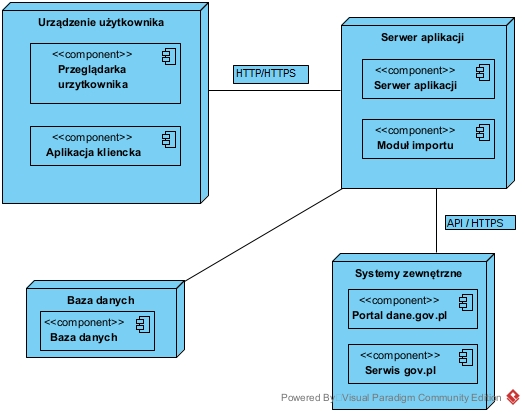
\includegraphics[width=0.75\linewidth]{Diagram_architektury_systemu}
\end{center}

System składa się z~następujących elementów:

\begin{itemize}
    \item \textbf{Przeglądarka użytkownika} -- uruchamia aplikację na
    telefonie lub komputerze (O-03). W~pamięci przeglądarki przechowywane są
    wybrana rola oraz lista ostatnio przeglądanych środków (WF-05, WF-15).
    \item \textbf{Aplikacja kliencka (frontend)} -- interfejs zaprojektowany
    w~podejściu \emph{Mobile First}. Wysyła zapytania do serwera i~prezentuje
    otrzymane wyniki.
    \item \textbf{Serwer aplikacji (API)} -- obsługuje wyszukiwanie,
    podpowiedzi, karty środków i~zamienniki. Zwraca wyłącznie dane potrzebne
    do wyświetlenia bieżącego widoku.
    \item \textbf{Baza danych} -- przechowuje dane rejestru i~historię
    wczytywania danych.
    \item \textbf{Moduł importu} -- proces uruchamiany codziennie przez
    harmonogram, niezależny od obsługi użytkowników. Pobiera nowe pliki przez
    API portalu dane.gov.pl i~wczytuje je do bazy danych.
    \item \textbf{Systemy zewnętrzne} -- portal dane.gov.pl (źródło danych,
    O-01) oraz serwis gov.pl, na którym publikowane są etykiety środków
    w~formacie PDF.
\end{itemize}

\subsubsection{Decyzje projektowe}

\begin{itemize}
    \item \textbf{Wyszukiwanie po stronie serwera.} Urządzenie użytkownika
    pobiera tylko wyniki zapytania, a~nie całą bazę środków, jak w~wyszukiwarce
    ministerstwa. Pozwala to spełnić WNF-01 i~WNF-02 również przy słabym
    zasięgu.
    \item \textbf{Brak uwierzytelniania.} System nie ma kont ani panelu
    administracyjnego (WNF-09, O-04), dlatego nie zawiera modułu logowania.
    Dane związane z~użytkownikiem pozostają na jego urządzeniu.
    \item \textbf{Wczytywanie danych w~całości albo wcale.} Moduł importu
    wczytuje nowe pliki do tabel tymczasowych, sprawdza ich poprawność,
    a~następnie w~jednej transakcji zastępuje nimi poprzednie dane. Błąd na
    dowolnym etapie pozostawia poprzednią wersję danych bez zmian (WNF-08).
    \item \textbf{Codzienne sprawdzanie publikacji.} Moduł importu porównuje
    datę publikacji plików na portalu z~datą ostatnio wczytanej wersji
    i~pobiera dane tylko wtedy, gdy pojawiła się nowa wersja. Codzienne
    sprawdzanie zapewnia spełnienie WNF-07 (najwyżej 7~dni od publikacji).
\end{itemize}

\subsubsection{Wybór technologii}

Na tym etapie wybrano wyłącznie system bazy danych, ponieważ wynika on
bezpośrednio z~charakteru danych i~wymagań. Pozostałe technologie zostaną
dobrane na etapie implementacji.

Wybrano bazę danych \textbf{PostgreSQL}, ponieważ:

\begin{itemize}
    \item dane rejestru mają charakter relacyjny -- środki, substancje czynne,
    zastosowania, uprawy i~agrofagi są ze sobą powiązane relacjami
    wiele-do-wielu, a~filtrowanie krzyżowe (WF-04) sprowadza się do złączeń
    tabel,
    \item standardowe rozszerzenia PostgreSQL realizują wyszukiwanie odporne
    na literówki (WF-02) bez osobnego silnika wyszukiwania: \emph{pg\_trgm}
    (indeks trigramowy, szybkie wyszukanie podobnych nazw),
    \emph{fuzzystrmatch} (odległość edycyjna, czyli sprawdzenie warunku
    ,,najwyżej 2~znaki'') oraz \emph{unaccent} (porównywanie nazw bez względu
    na polskie znaki),
    \item transakcje obejmujące wiele tabel pozwalają zrealizować podmianę
    danych w~całości albo wcale (WNF-08).
\end{itemize}

\subsection{Moduły systemu}

\begingroup
\small
\begin{longtable}{|>{\raggedright\arraybackslash}p{3cm}|p{9.4cm}|>{\raggedright\arraybackslash}p{2.2cm}|}
\hline
\textbf{Moduł} & \textbf{Odpowiedzialność} & \textbf{Wymagania} \\
\hline
\endfirsthead
\hline
\textbf{Moduł} & \textbf{Odpowiedzialność} & \textbf{Wymagania} \\
\hline
\endhead
Wyszukiwanie &
Wyszukiwanie środków po nazwie handlowej i~substancji czynnej z~tolerancją
literówek, filtrowanie krzyżowe po uprawie, agrofagu i~rodzaju środka,
ograniczenie wyników do wybranej roli, informacja o~środkach usuniętych
z~rejestru. &
WF-01 -- WF-05, WF-12 \\
\hline
Podpowiedzi słownikowe &
Podpowiadanie nazw upraw, agrofagów, substancji czynnych i~rodzajów środków
podczas wpisywania, z~tolerancją literówek. Wybrana pozycja jest przekazywana
do wyszukiwania jako jednoznaczny identyfikator. &
WF-02 -- WF-04 \\
\hline
Karta środka &
Prezentacja danych środka i~wszystkich jego zastosowań, okresu karencji lub
odnośnika do etykiety, oznaczenia upływającego terminu dopuszczenia oraz
stałego adresu karty. &
WF-06, WF-07, WF-08, WF-11, WF-16 \\
\hline
Zamienniki &
Wyszukiwanie środków o~tych samych substancjach czynnych, sortowanie według
zgodności zawartości, filtrowanie według uprawy i~roli, pomijanie środków,
których termin dopuszczenia do stosowania upłynął. &
WF-05, WF-10 \\
\hline
Etykiety &
Wyświetlanie etykiety w~aplikacji i~jej pobieranie na urządzenie. &
WF-09 \\
\hline
Import danych &
Sprawdzanie publikacji na portalu, pobieranie plików, kontrola ich
poprawności, ujednolicanie nazw, wczytanie i~podmiana danych, zapis
przebiegu i~błędów w~dzienniku zdarzeń. &
WF-13, WF-14, WNF-07, WNF-08 \\
\hline
Preferencje lokalne &
Zapamiętywanie roli i~listy 10 ostatnio przeglądanych środków w~pamięci
przeglądarki (część aplikacji klienckiej). &
WF-05, WF-15 \\
\hline
\end{longtable}
\endgroup

\subsection{Aktorzy i~przypadki użycia}

\begin{itemize}
    \item \textbf{Użytkownik} -- osoba korzystająca z~aplikacji bez konta.
    Występuje w~jednej z~dwóch ról: \textbf{użytkownik profesjonalny} lub
    \textbf{użytkownik nieprofesjonalny}. Obie role mają te same przypadki
    użycia, a~rola wpływa jedynie na zakres prezentowanych środków.
    \item \textbf{Harmonogram} -- aktor systemowy, który codziennie uruchamia
    aktualizację danych.
    \item \textbf{Portal dane.gov.pl} -- system zewnętrzny udostępniający
    pliki rejestru.
\end{itemize}

\begingroup
\small
\begin{longtable}{|p{1.3cm}|>{\raggedright\arraybackslash}p{6.1cm}|>{\raggedright\arraybackslash}p{3cm}|>{\raggedright\arraybackslash}p{3.7cm}|}
\hline
\textbf{ID} & \textbf{Przypadek użycia} & \textbf{Aktor} & \textbf{Wymagania} \\
\hline
\endfirsthead
\hline
\textbf{ID} & \textbf{Przypadek użycia} & \textbf{Aktor} & \textbf{Wymagania} \\
\hline
\endhead
PU-01 & Wyszukaj środek po nazwie & Użytkownik & WF-01, WF-02, WF-12 \\
\hline
PU-02 & Wyszukaj środki po substancji czynnej & Użytkownik & WF-02, WF-03 \\
\hline
PU-03 & Znajdź środek na agrofaga w~uprawie & Użytkownik & WF-02, WF-04, WF-05 \\
\hline
PU-04 & Wybierz rolę & Użytkownik & WF-05 \\
\hline
PU-05 & Przeglądaj kartę środka & Użytkownik & WF-06, WF-07, WF-08, WF-11 \\
\hline
PU-06 & Wyświetl lub pobierz etykietę & Użytkownik & WF-09 \\
\hline
PU-07 & Znajdź zamienniki środka & Użytkownik & WF-05, WF-10 \\
\hline
PU-08 & Przeglądaj ostatnio oglądane środki & Użytkownik & WF-15 \\
\hline
PU-09 & Udostępnij kartę środka & Użytkownik & WF-16 \\
\hline
PU-10 & Zaktualizuj dane z~rejestru & Harmonogram, portal dane.gov.pl &
WF-13, WF-14, WNF-07, WNF-08 \\
\hline
\end{longtable}
\endgroup

\begin{center}
    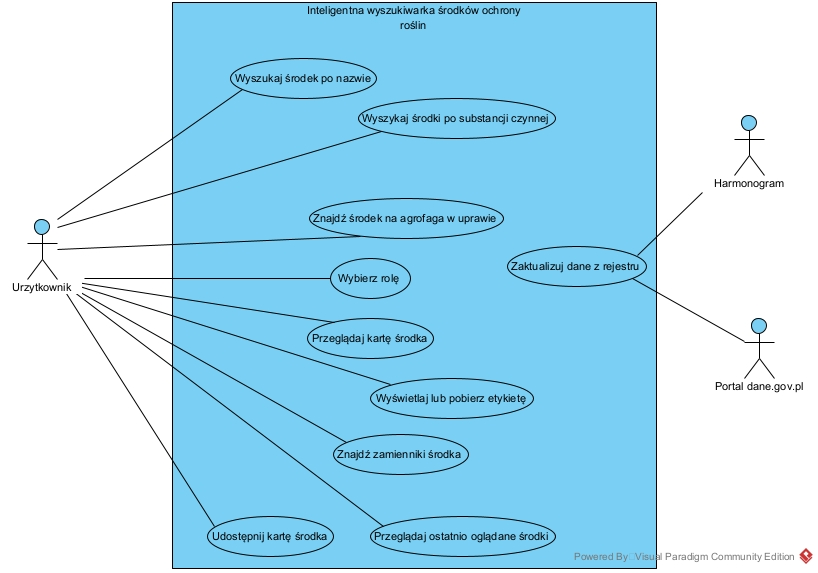
\includegraphics[width=\linewidth]{diagram_przypadkow_uzycia}
\end{center}

\subsection{Scenariusz: znalezienie środka na agrofaga w~uprawie}

Jako najważniejszą operację wybrano przypadek PU-03, ponieważ odpowiada on na
podstawowe pytanie wszystkich grup użytkowników: czym można zwalczać danego
agrofaga w~danej uprawie.

\textbf{Aktor:} użytkownik (profesjonalny lub nieprofesjonalny).

\textbf{Warunki początkowe:} w~systemie jest wczytana co najmniej jedna wersja
danych rejestru, a~użytkownik ma wybraną rolę (PU-04). Przy pierwszym
uruchomieniu aplikacja prosi o~jej wybór.

\textbf{Scenariusz główny:}

\begin{enumerate}
    \item Użytkownik otwiera wyszukiwarkę. System wyświetla formularz
    wyszukiwania, wybraną rolę oraz datę publikacji wersji danych (WF-14).
    \item Użytkownik wpisuje co najmniej 3 znaki nazwy uprawy, np.
    ,,ziemn''.
    \item System podpowiada pasujące uprawy ze słownika, również wtedy, gdy
    wpisana nazwa zawiera literówkę (WF-02).
    \item Użytkownik wybiera uprawę ,,ziemniak''. Kroki 2--4 powtarza dla
    agrofaga (,,stonka ziemniaczana'') i~opcjonalnie dla rodzaju środka.
    \item Aplikacja wysyła do serwera identyfikatory wybranych pozycji oraz
    rolę użytkownika.
    \item Serwer wybiera zastosowania spełniające wszystkie kryteria
    i~zwraca listę, w~której każdy środek występuje jeden raz (WF-04).
    W~roli nieprofesjonalnej lista obejmuje wyłącznie środki dopuszczone dla
    użytkowników nieprofesjonalnych (WF-05).
    \item System wyświetla listę środków z~nazwą, substancjami czynnymi,
    rodzajem środka i~oznaczeniem upływającego terminu dopuszczenia (WF-11).
    \item Użytkownik wybiera środek, a~system wyświetla jego kartę (PU-05).
\end{enumerate}

\textbf{Warunek końcowy:} użytkownik widzi kartę środka dopuszczonego do
zwalczania wybranego agrofaga w~wybranej uprawie.

\textbf{Scenariusze alternatywne i~sytuacje błędne:}

\begin{itemize}
    \item \textbf{3a. Brak pasującej nazwy w~słowniku.} Wpisana nazwa różni
    się od wszystkich nazw w~słowniku o~więcej niż 2 znaki. System informuje,
    że nie znaleziono takiej uprawy (lub agrofaga), a~użytkownik poprawia nazwę --
    powrót do kroku 2.
    \item \textbf{5a. Brak połączenia z~serwerem.} Aplikacja wyświetla
    komunikat o~braku połączenia, zachowuje wybrane filtry i~udostępnia
    przycisk ponowienia zapytania.
    \item \textbf{6a. Brak środków spełniających wszystkie kryteria.} System
    wyświetla komunikat o~braku wyników i~listę wybranych filtrów, z~których
    każdy można usunąć jednym dotknięciem (kryterium akceptacji WF-04).
    \item \textbf{6b. Brak środków dla roli nieprofesjonalnej.} Kryteria
    spełniają wyłącznie środki dla użytkowników profesjonalnych. System
    informuje, że dla tej uprawy i~agrofaga nie ma środków dopuszczonych dla
    użytkowników nieprofesjonalnych.
    \item \textbf{6c. Trwa lub nie powiodła się aktualizacja danych.}
    Zapytanie jest obsługiwane na poprzedniej wersji danych (WNF-08),
    a~na ekranie widnieje data jej publikacji (WF-14).
\end{itemize}

\subsection{Model danych}

\begin{center}
    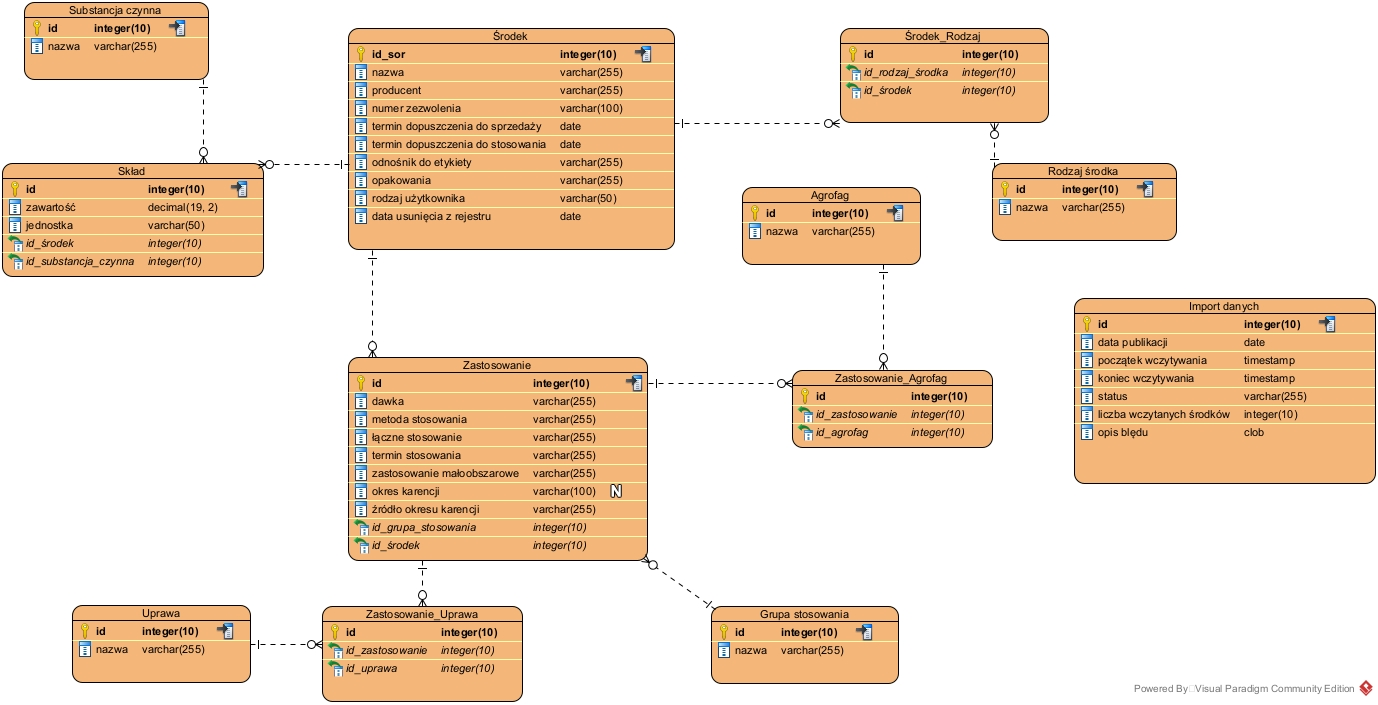
\includegraphics[width=\linewidth]{Diagram_erd}
\end{center}

Model danych odwzorowuje pliki rejestru publikowane na portalu dane.gov.pl:
rejestr podstawowy, rejestr zastosowań, rejestr kart środków, słowniki oraz
wykaz środków usuniętych z~rejestru.

\subsubsection{Decyzje dotyczące modelu}

\begin{itemize}
    \item \textbf{Jedno zastosowanie odpowiada jednemu wierszowi rejestru
    zastosowań.} Wiersz rejestru wymienia często kilka upraw i~kilkanaście
    agrofagów o~wspólnej dawce i~terminie, dlatego uprawy i~agrofagi są
    powiązane z~zastosowaniem relacjami wiele-do-wielu. Rozpisanie każdej pary
    uprawa--agrofag jako osobnego zastosowania zwiększyłoby liczbę rekordów
    z~ok.~18\,700 do ponad 158\,000.
    \item \textbf{Zastosowanie może nie mieć agrofaga.} W~rejestrze występują
    zastosowania bez wskazanego agrofaga, np. regulatorów wzrostu. Wymaganie
    agrofaga spowodowałoby pominięcie takich środków w~wynikach wyszukiwania po
    uprawie.
    \item \textbf{Zawartość substancji czynnej jako liczba z~jednostką.}
    Rejestr podaje skład w~postaci tekstu (np. ,,azoksystrobina -- 250~g'').
    Zapis liczbowy pozwala ustawić zamienniki o~tej samej zawartości na
    początku listy (WF-10).
    \item \textbf{Okres karencji jako pole opcjonalne.} Okres karencji jest
    podany tylko w~części opisów terminu stosowania (O-01). Puste pole oznacza,
    że karta środka kieruje do etykiety (WF-07), a~źródło okresu karencji
    pozwala w~przyszłości uzupełnić go danymi z~etykiet (WF-08).
    \item \textbf{Data usunięcia zamiast usuwania rekordu.} Środek usunięty
    z~rejestru pozostaje w~bazie z~datą usunięcia, dzięki czemu jego wyszukanie
    zwraca informację o~usunięciu (WF-12).
    \item \textbf{Indeksy trigramowe} na nazwach środków, substancji czynnych,
    upraw i~agrofagów przyspieszają wyszukiwanie z~tolerancją literówek
    (WF-02, WNF-01).
    \item \textbf{Dane użytkownika poza bazą.} Rola i~ostatnio przeglądane
    środki są zapisywane wyłącznie w~przeglądarce, dlatego nie występują
    w~modelu danych (WNF-09).
\end{itemize}

\subsection{Projekt najważniejszych ekranów}

Wszystkie ekrany projektowane są najpierw dla telefonu o~szerokości 360
pikseli (WNF-03), z~elementami dotykowymi o~wymiarach co najmniej
$48 \times 48$ pikseli (WNF-04), kontrastem co najmniej 7:1 (WNF-05)
i~nazewnictwem zgodnym z~rejestrem (WNF-10).

\subsubsection{E-1: Wyszukiwarka}

\begin{center}
    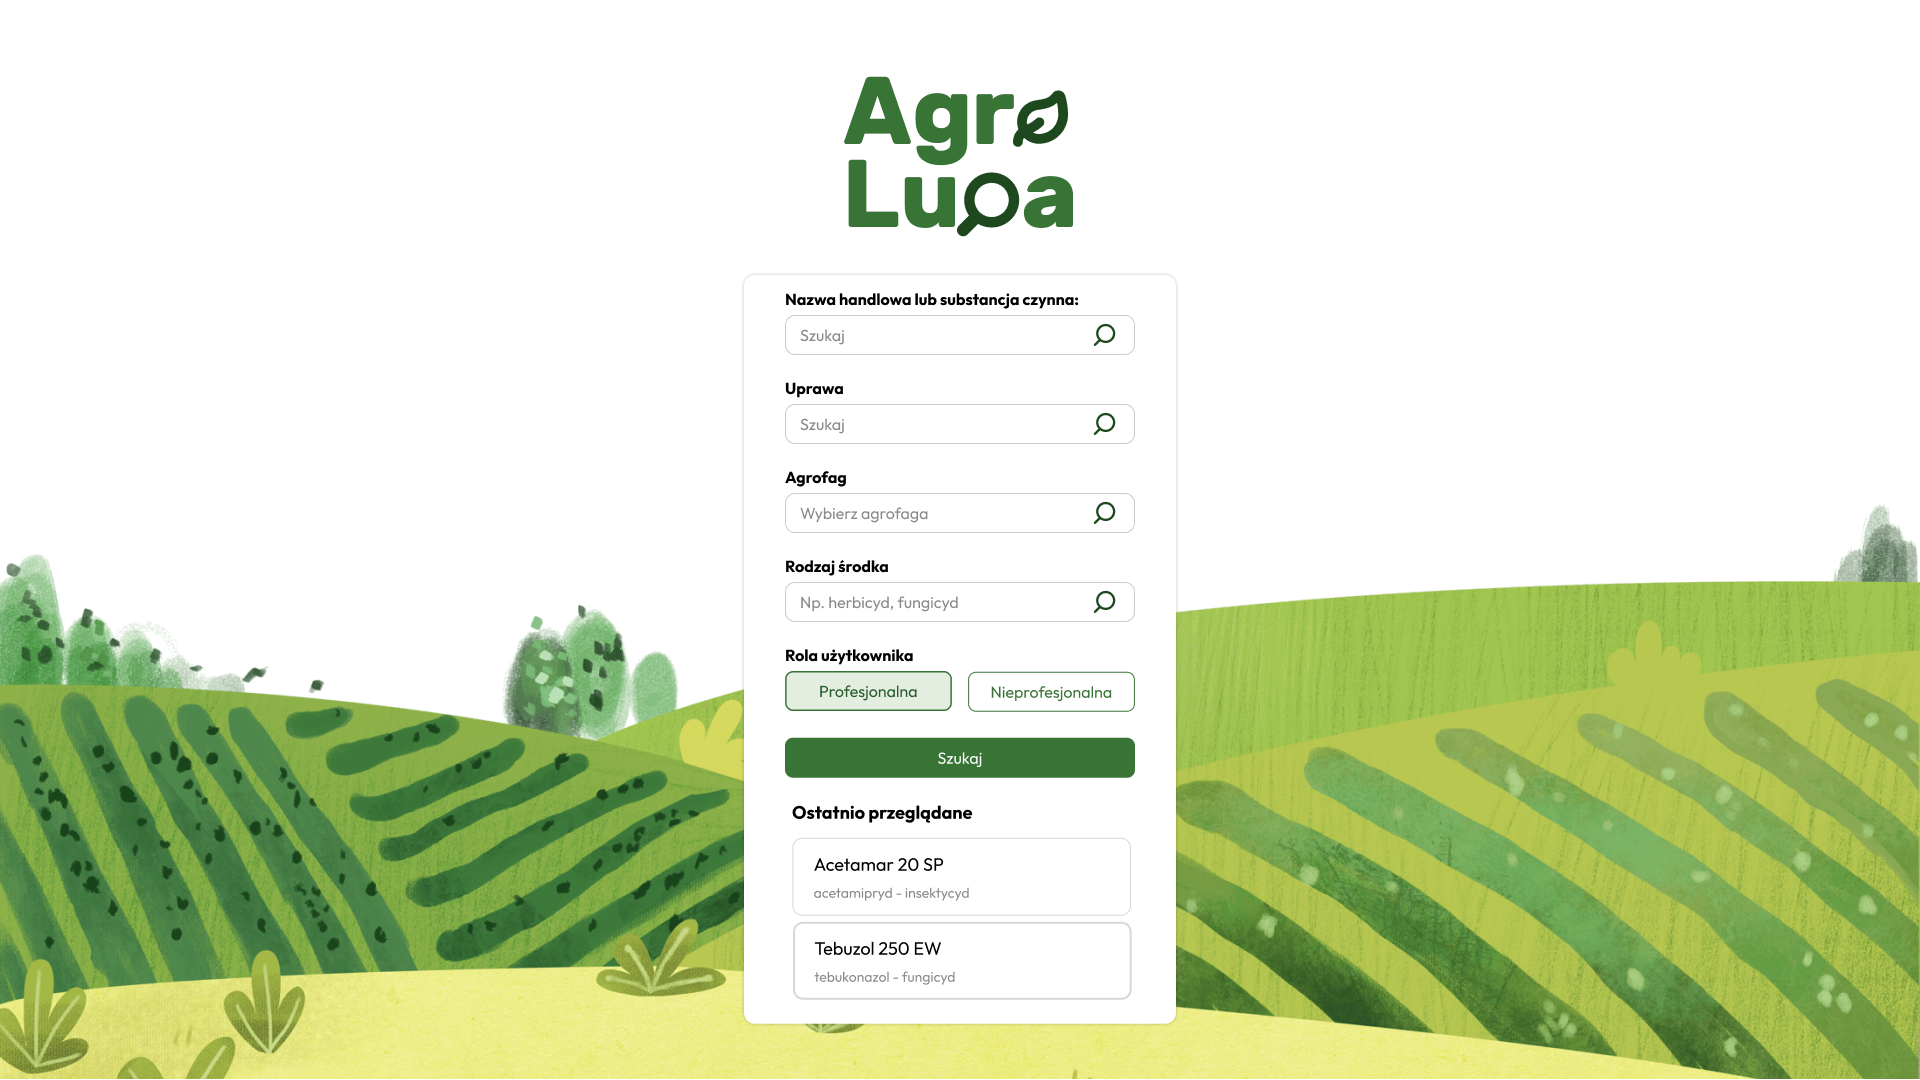
\includegraphics[width=\linewidth]{E-1_Wyszukiwarka}
\end{center}

\begin{itemize}
    \item pole wyszukiwania nazwy handlowej lub substancji czynnej,
    \item pola uprawy, agrofaga i~rodzaju środka z~podpowiedziami; wybrane
    pozycje wyświetlane są jako etykiety z~przyciskiem usunięcia,
    \item przełącznik roli: profesjonalna / nieprofesjonalna,
    \item lista ostatnio przeglądanych środków (WF-15),
    \item data publikacji wersji danych (WF-14).
\end{itemize}

\subsubsection{E-2: Lista wyników}

\begin{center}
    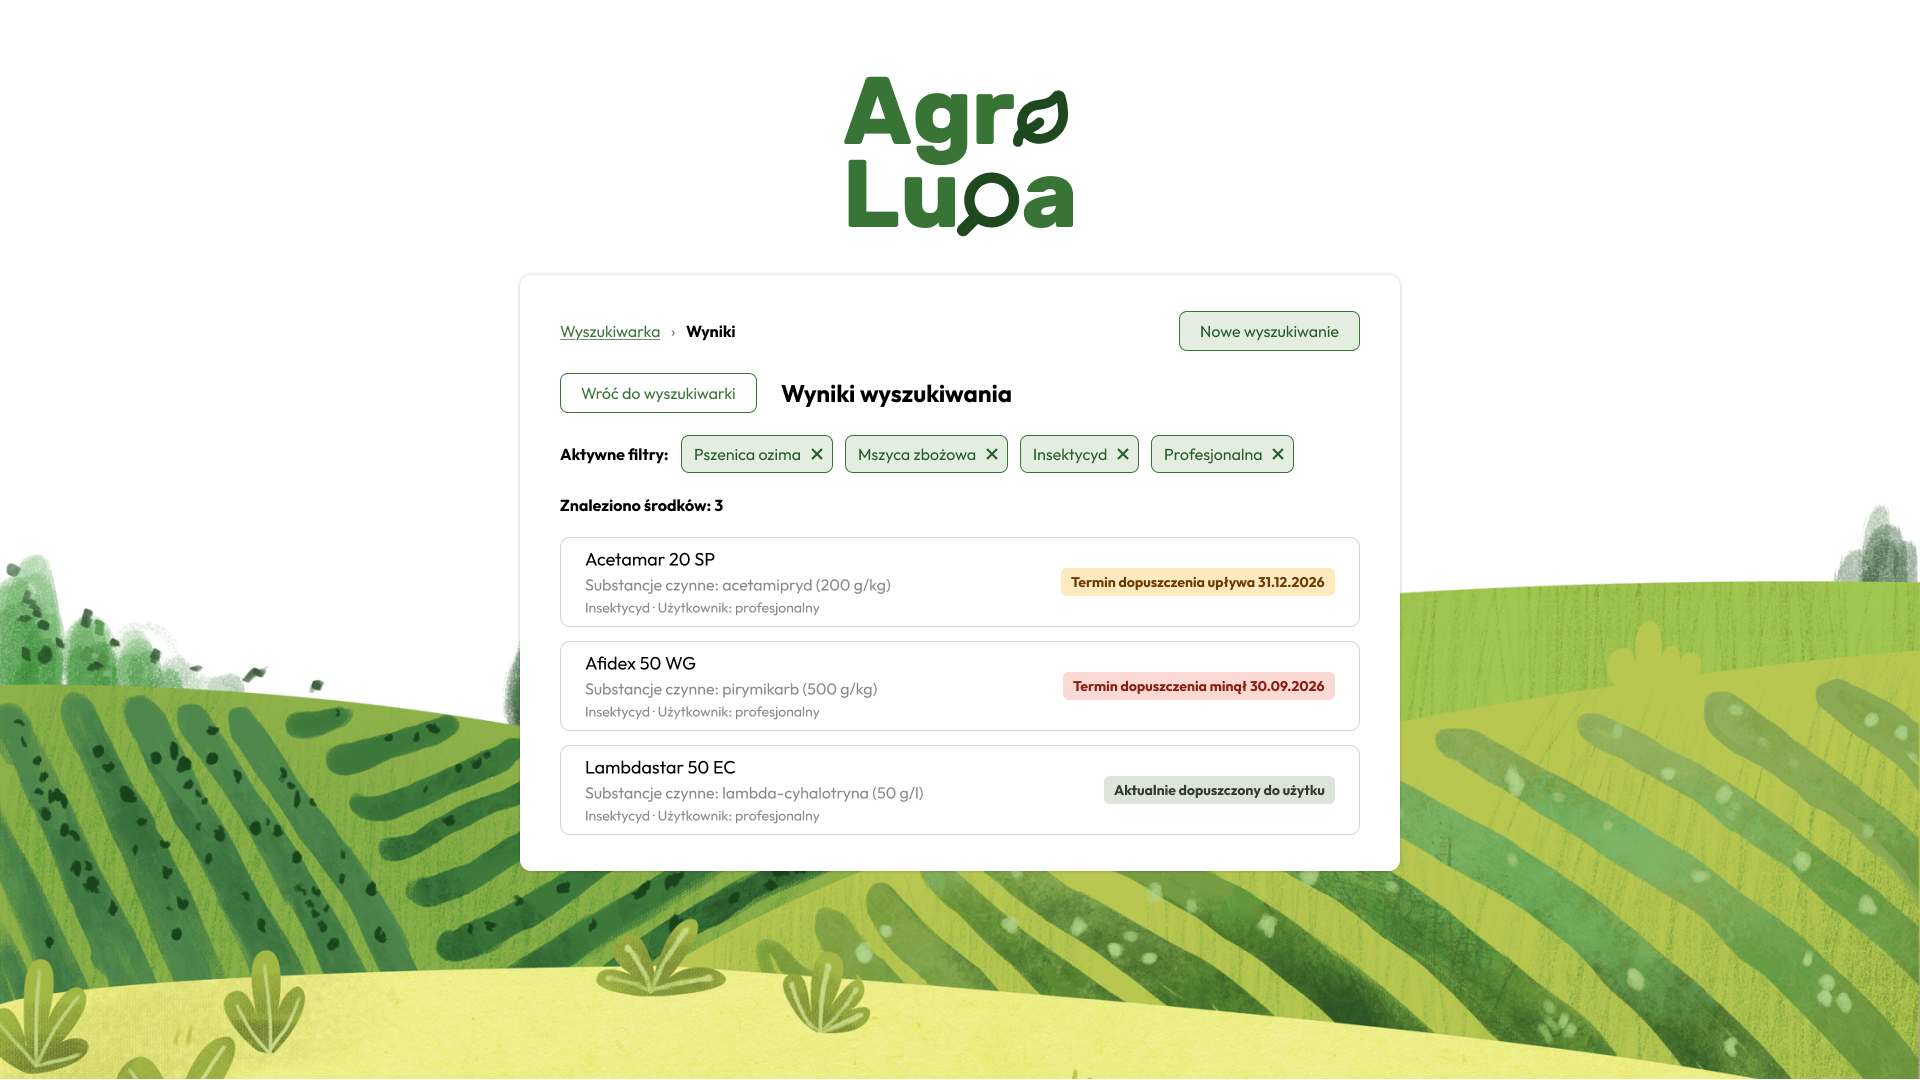
\includegraphics[width=\linewidth]{E-2_Lista_wynikow}
\end{center}

\begin{itemize}
    \item aktywne filtry z~możliwością usunięcia każdego z~nich,
    \item liczba znalezionych środków,
    \item dla każdego środka: nazwa, substancje czynne, rodzaj środka, rodzaj
    użytkownika oraz oznaczenie upływającego lub minionego terminu
    dopuszczenia (WF-11),
    \item komunikaty: brak wyników, brak środków dla roli nieprofesjonalnej,
    środek usunięty z~rejestru wraz z~datą (WF-12).
\end{itemize}

Ekran E-2 w~przypadku braku wyników:

\begin{center}
    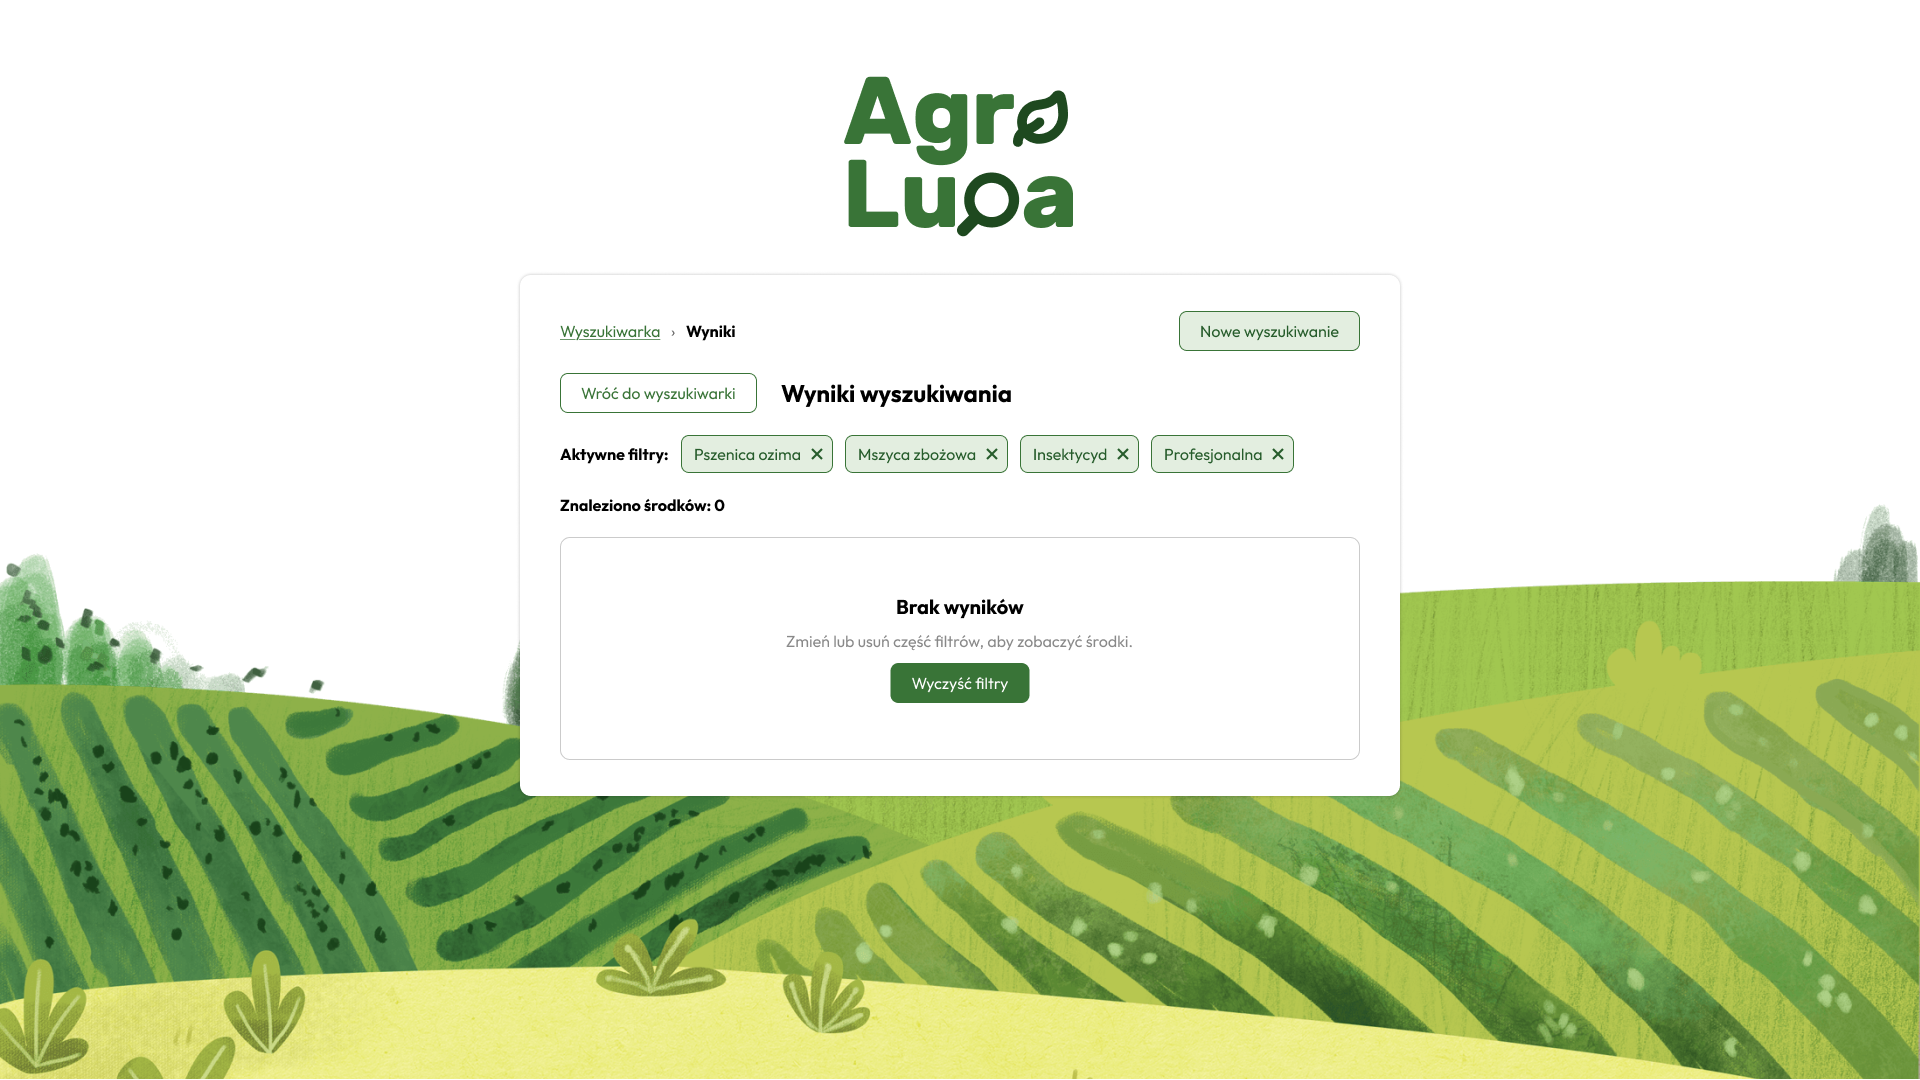
\includegraphics[width=\linewidth]{E-2_Lista_wynikow_brak_wynikow}
\end{center}

\subsubsection{E-3: Karta środka}

\begin{center}
    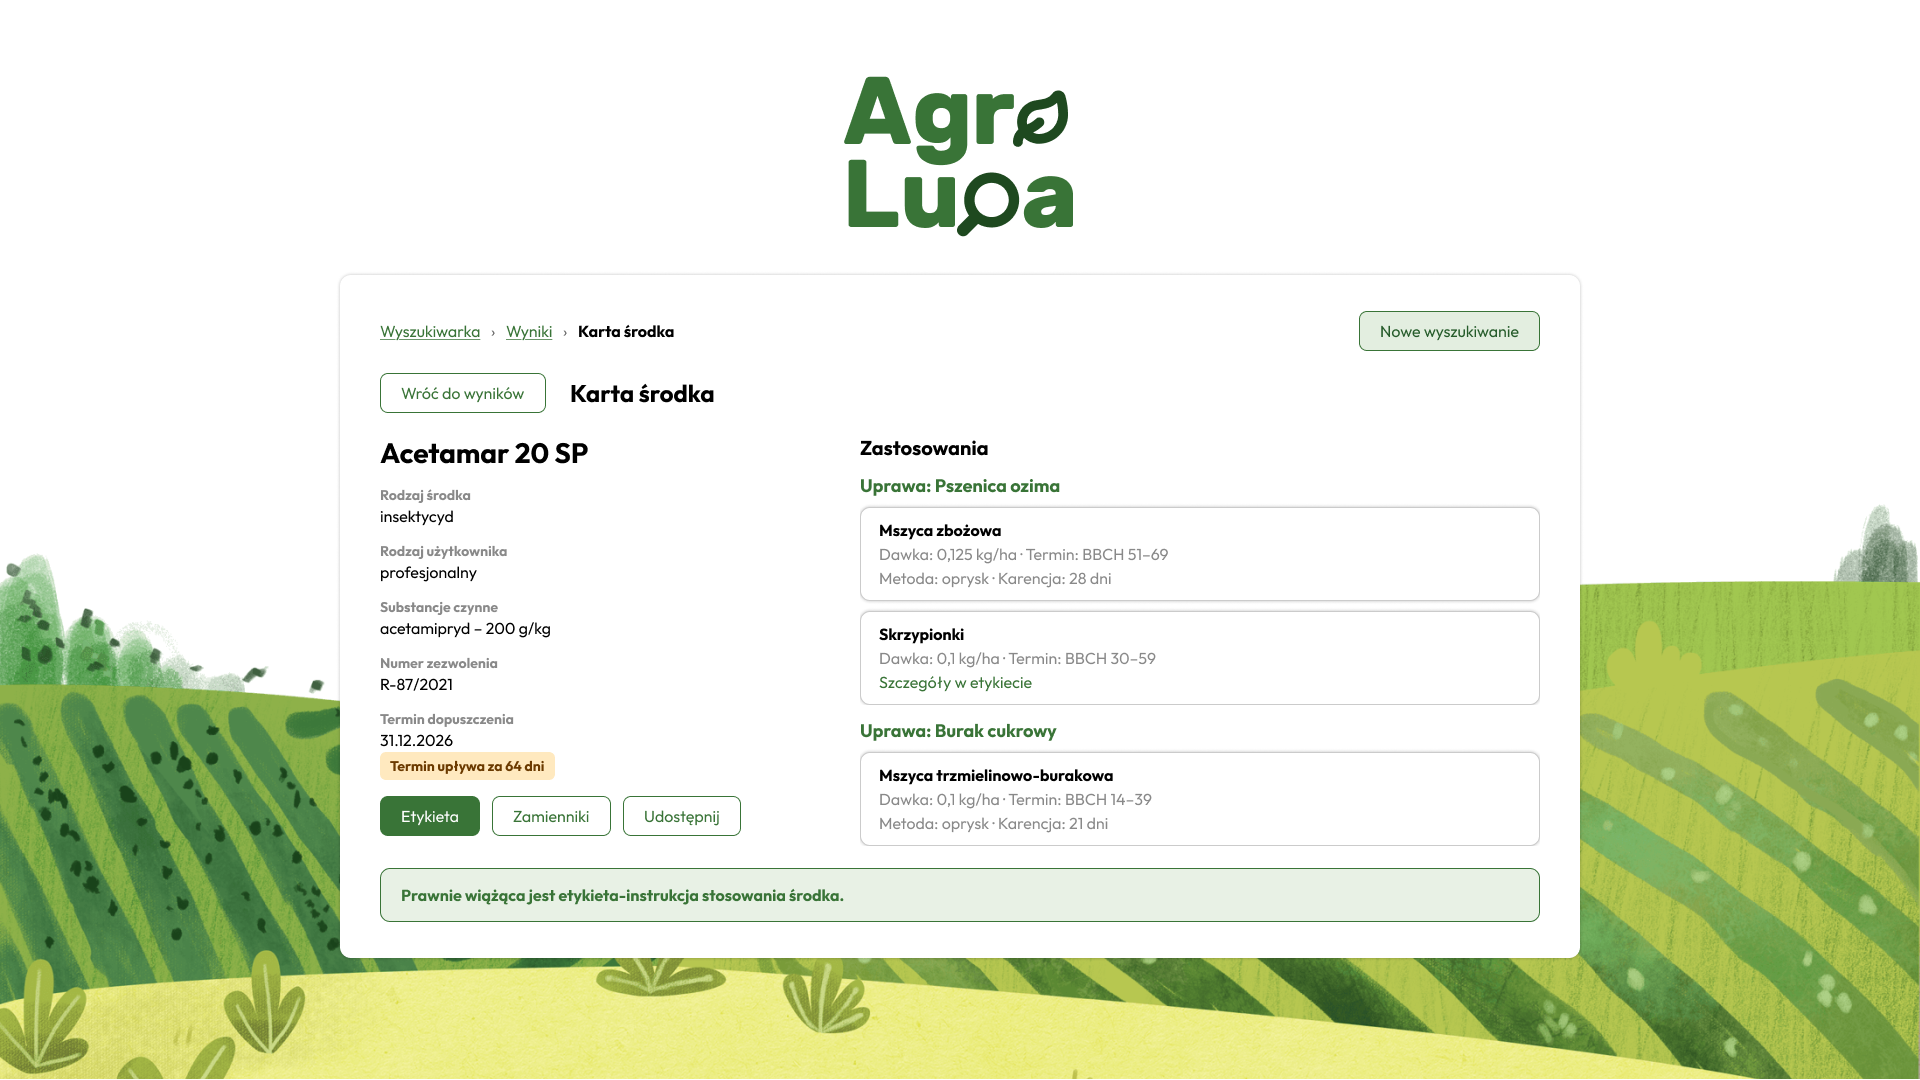
\includegraphics[width=\linewidth]{E-3_Karta_srodka}
\end{center}

\begin{itemize}
    \item dane środka zgodnie z~WF-06 oraz terminy z~oznaczeniem upływającego
    terminu (WF-11),
    \item lista zastosowań pogrupowana według upraw: agrofag, dawka, termin,
    metoda stosowania i~okres karencji lub odnośnik do etykiety (WF-07),
    \item przyciski: ,,Etykieta'', ,,Zamienniki'', ,,Udostępnij'' (WF-09,
    WF-10, WF-16),
    \item stała informacja, że prawnie wiążąca jest etykieta-instrukcja
    stosowania środka (O-02).
\end{itemize}

\subsubsection{E-4: Zamienniki}

\begin{center}
    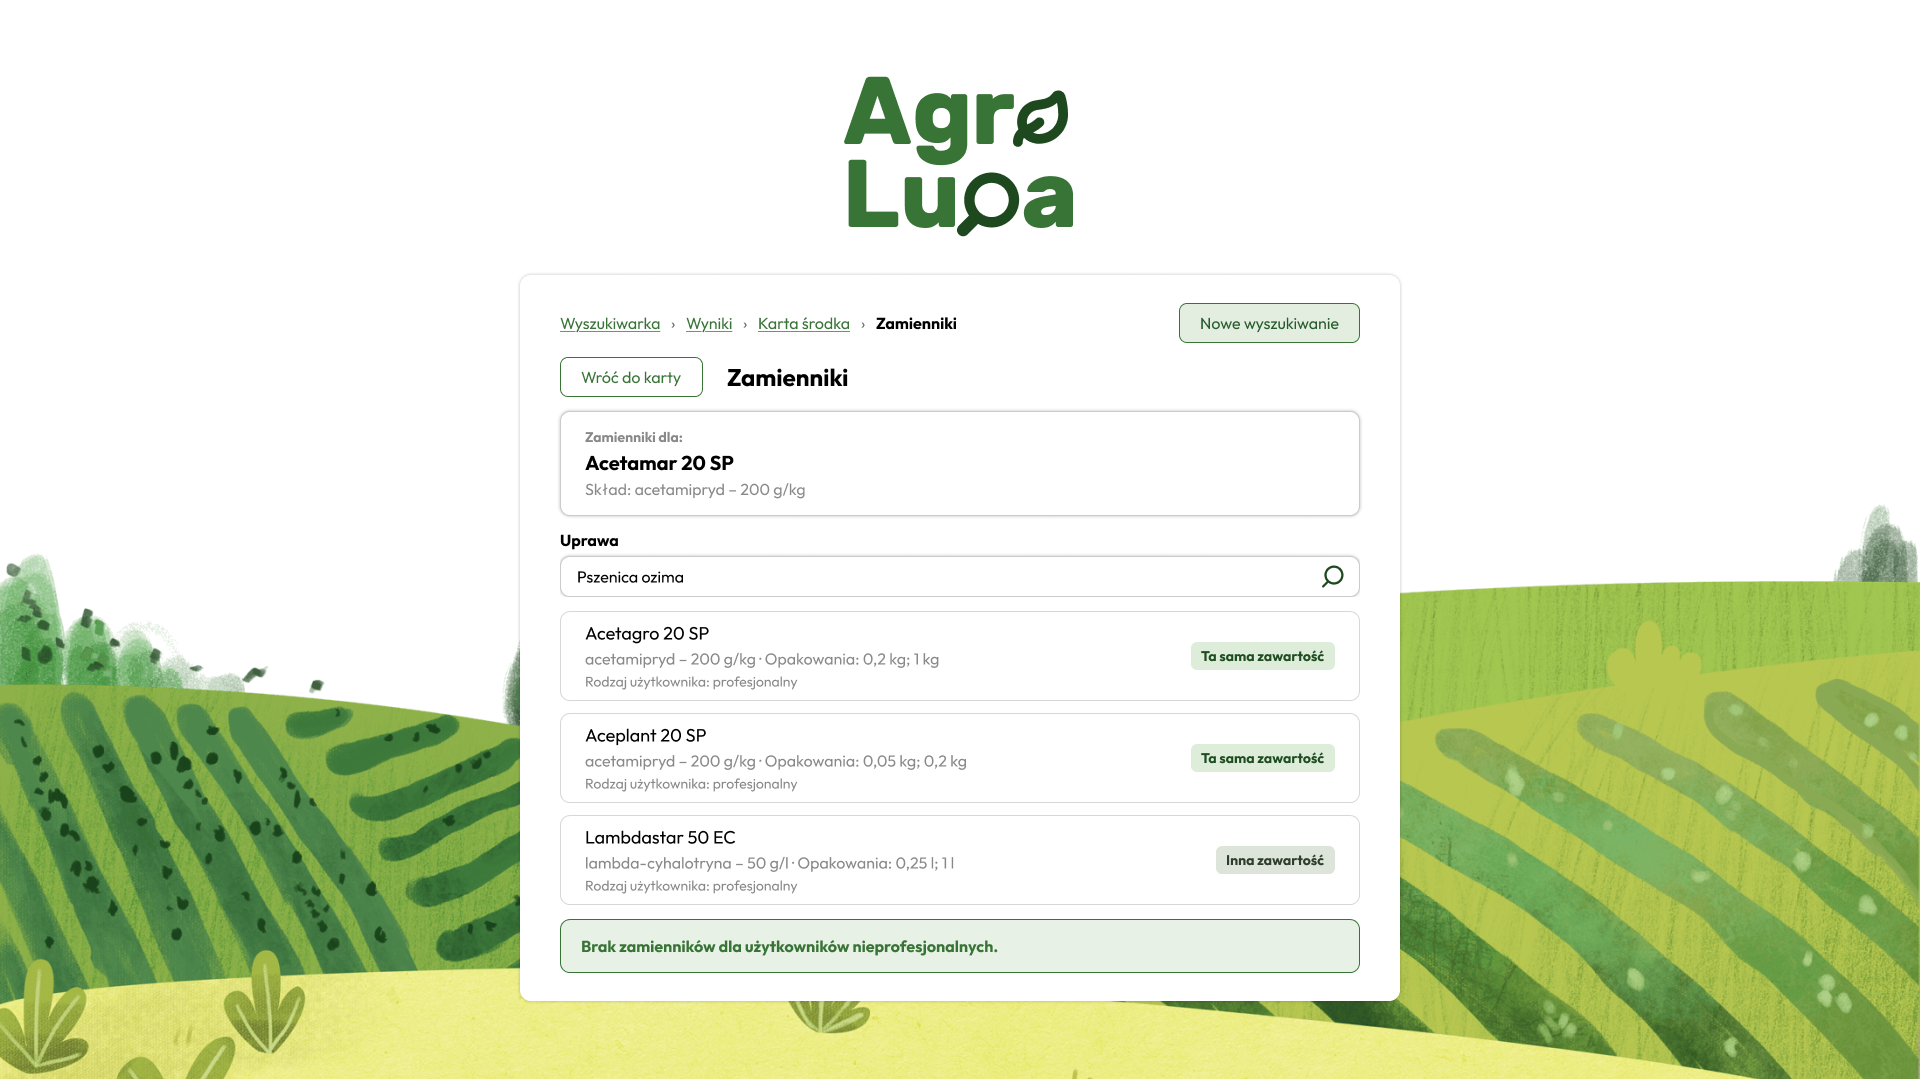
\includegraphics[width=\linewidth]{E-4_Zamienniki}
\end{center}

\begin{itemize}
    \item nazwa i~skład środka, dla którego wyszukano zamienniki,
    \item filtr uprawy,
    \item lista zamienników z~zawartością substancji czynnej, opakowaniami
    i~rodzajem użytkownika; środki o~tej samej zawartości na początku (WF-10),
    \item komunikat o~braku zamienników dla użytkowników nieprofesjonalnych.
\end{itemize}

\subsubsection{E-5: Podgląd etykiety}

\begin{center}
    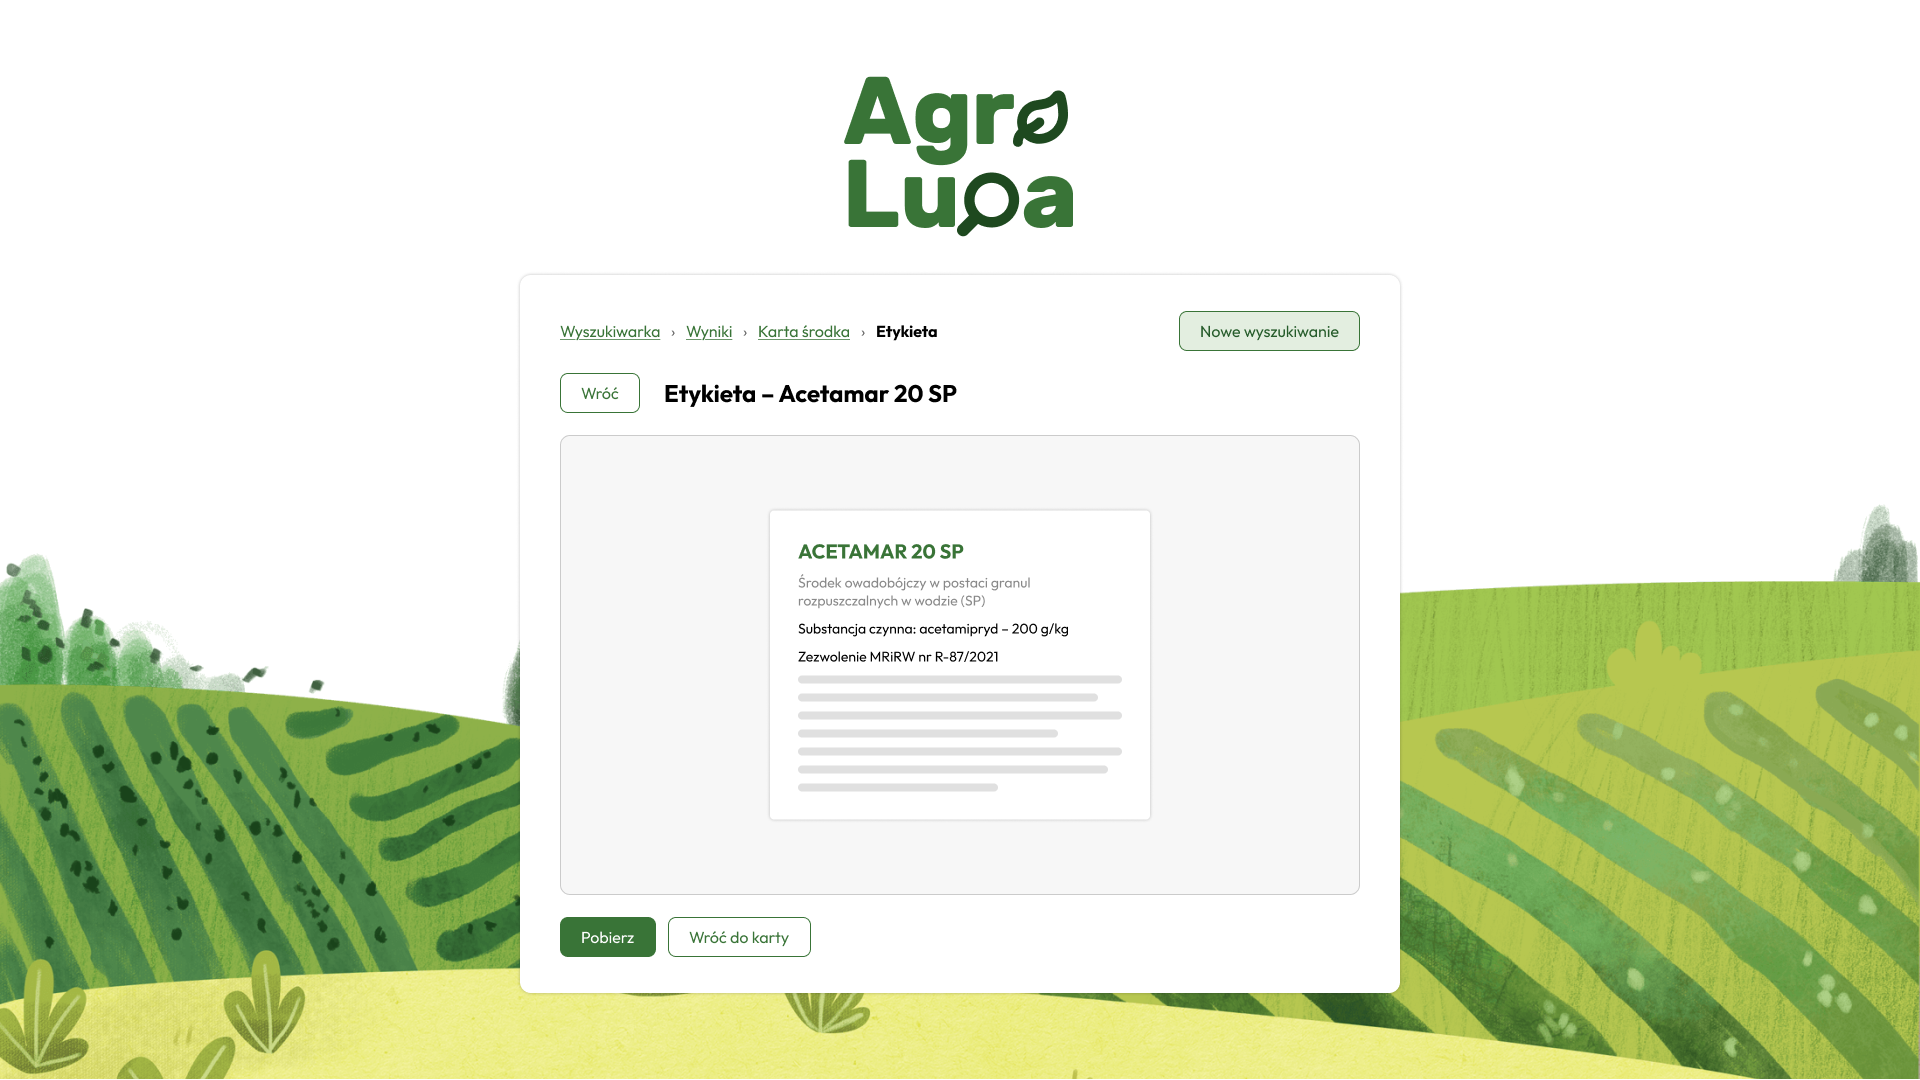
\includegraphics[width=\linewidth]{E-5_Podglad_etykiety}
\end{center}

\begin{itemize}
    \item etykieta wyświetlana w~aplikacji z~przyciskami ,,Pobierz''
    i~,,Wróć do karty'' (WF-09).
\end{itemize}

\subsection{Powiązanie z~wymaganiami}
\label{sec:powiazanie}

\begingroup
\small
\begin{longtable}{|p{1.7cm}|>{\raggedright\arraybackslash}p{2cm}|>{\raggedright\arraybackslash}p{3.3cm}|>{\raggedright\arraybackslash}p{1.6cm}|>{\raggedright\arraybackslash}p{5cm}|}
\hline
\textbf{Wymag.} & \textbf{Przypadek użycia} & \textbf{Moduł} & \textbf{Ekran} & \textbf{Dane i~inne elementy projektu} \\
\hline
\endfirsthead
\hline
\textbf{Wymag.} & \textbf{Przypadek użycia} & \textbf{Moduł} & \textbf{Ekran} & \textbf{Dane i~inne elementy projektu} \\
\hline
\endhead
WF-01 & PU-01 & Wyszukiwanie & E-1, E-2 & Środek \\
\hline
WF-02 & PU-01 -- PU-03 & Wyszukiwanie, Podpowiedzi & E-1 & indeksy trigramowe, pg\_trgm, fuzzystrmatch, unaccent \\
\hline
WF-03 & PU-02 & Wyszukiwanie & E-1, E-2 & Substancja czynna, Skład \\
\hline
WF-04 & PU-03 & Wyszukiwanie, Podpowiedzi & E-1, E-2 & Zastosowanie, Uprawa, Agrofag, Rodzaj środka \\
\hline
WF-05 & PU-03, PU-04, PU-07 & Wyszukiwanie, Zamienniki, Preferencje & E-1, E-2, E-4 & Środek: rodzaj użytkownika \\
\hline
WF-06 & PU-05 & Karta środka & E-3 & Środek, Skład, Zastosowanie \\
\hline
WF-07 & PU-05 & Karta środka & E-3 & Zastosowanie: okres karencji \\
\hline
WF-08 & PU-05 & Karta środka & E-3 & Zastosowanie: źródło okresu karencji \\
\hline
WF-09 & PU-06 & Etykiety & E-5 & Środek: odnośnik do etykiety \\
\hline
WF-10 & PU-07 & Zamienniki & E-4 & Skład: zawartość i~jednostka \\
\hline
WF-11 & PU-03, PU-05 & Karta środka & E-2, E-3 & Środek: terminy dopuszczenia \\
\hline
WF-12 & PU-01 & Wyszukiwanie & E-2 & Środek: data usunięcia z~rejestru \\
\hline
WF-13 & PU-10 & Import danych & -- & Import danych \\
\hline
WF-14 & PU-10 & Import danych & E-1 & Import danych: data publikacji \\
\hline
WF-15 & PU-08 & Preferencje & E-1 & pamięć przeglądarki \\
\hline
WF-16 & PU-09 & Karta środka & E-3 & stały adres oparty na id\_sor \\
\hline
WNF-01 & PU-01 -- PU-03 & Wyszukiwanie & -- & wyszukiwanie po stronie serwera, indeksy \\
\hline
WNF-02 & -- & Aplikacja kliencka & -- & przesyłanie wyłącznie wyników \\
\hline
WNF-03 --\newline WNF-05 &-- & Aplikacja kliencka & wszystkie & zasady projektowania ekranów \\
\hline
WNF-06 & -- & Aplikacja kliencka & wszystkie & aplikacja przeglądarkowa (O-03) \\
\hline
WNF-07 & PU-10 & Import danych & -- & codzienne sprawdzanie publikacji \\
\hline
WNF-08 & PU-10 & Import danych & -- & podmiana danych w~jednej transakcji, Import danych \\
\hline
WNF-09 & -- & -- & -- & brak uwierzytelniania, dane użytkownika w~przeglądarce \\
\hline
WNF-10 & -- & Aplikacja kliencka & wszystkie & nazewnictwo pól zgodne z~rejestrem \\
\hline
\end{longtable}
\endgroup


\newpage
\section{Wstępny podział prac}

Prace nad projektem zostaną podzielone pomiędzy trzech członków
zespołu.

\begin{itemize}

    \item
    \textbf{Jakub Bakaj -- baza danych i~przetwarzanie danych:}
    projekt schematu relacyjnej bazy danych oraz wdrożenie procesu
    automatycznej aktualizacji danych (Worker/Cron) z~plików CSV/XLSX
    pobieranych przez API portalu dane.gov.pl.

    \item
    \textbf{Natalia Duda -- backend:}
    przygotowanie punktów końcowych (API) wyszukiwarki oraz ich integracja
    z~interfejsem użytkownika.

    \item
    \textbf{Damian Nowak -- frontend i UX:}
    zaprojektowanie i wdrożenie responsywnego interfejsu
    użytkownika, integracja formularzy wyszukiwania z API oraz
    implementacja karty szczegółów produktu.

\end{itemize}

\end{document}